\chapter{Supporting Screenshots}

This appendix contains screenshots of the developed web application for both
desktop (1920x1080) and mobile (1290x2796) layouts. For clarity, each screen
is shown in its desktop version first, followed by the corresponding mobile version.

\section{Wireframes}

\begin{figure}[H]
    \centering
    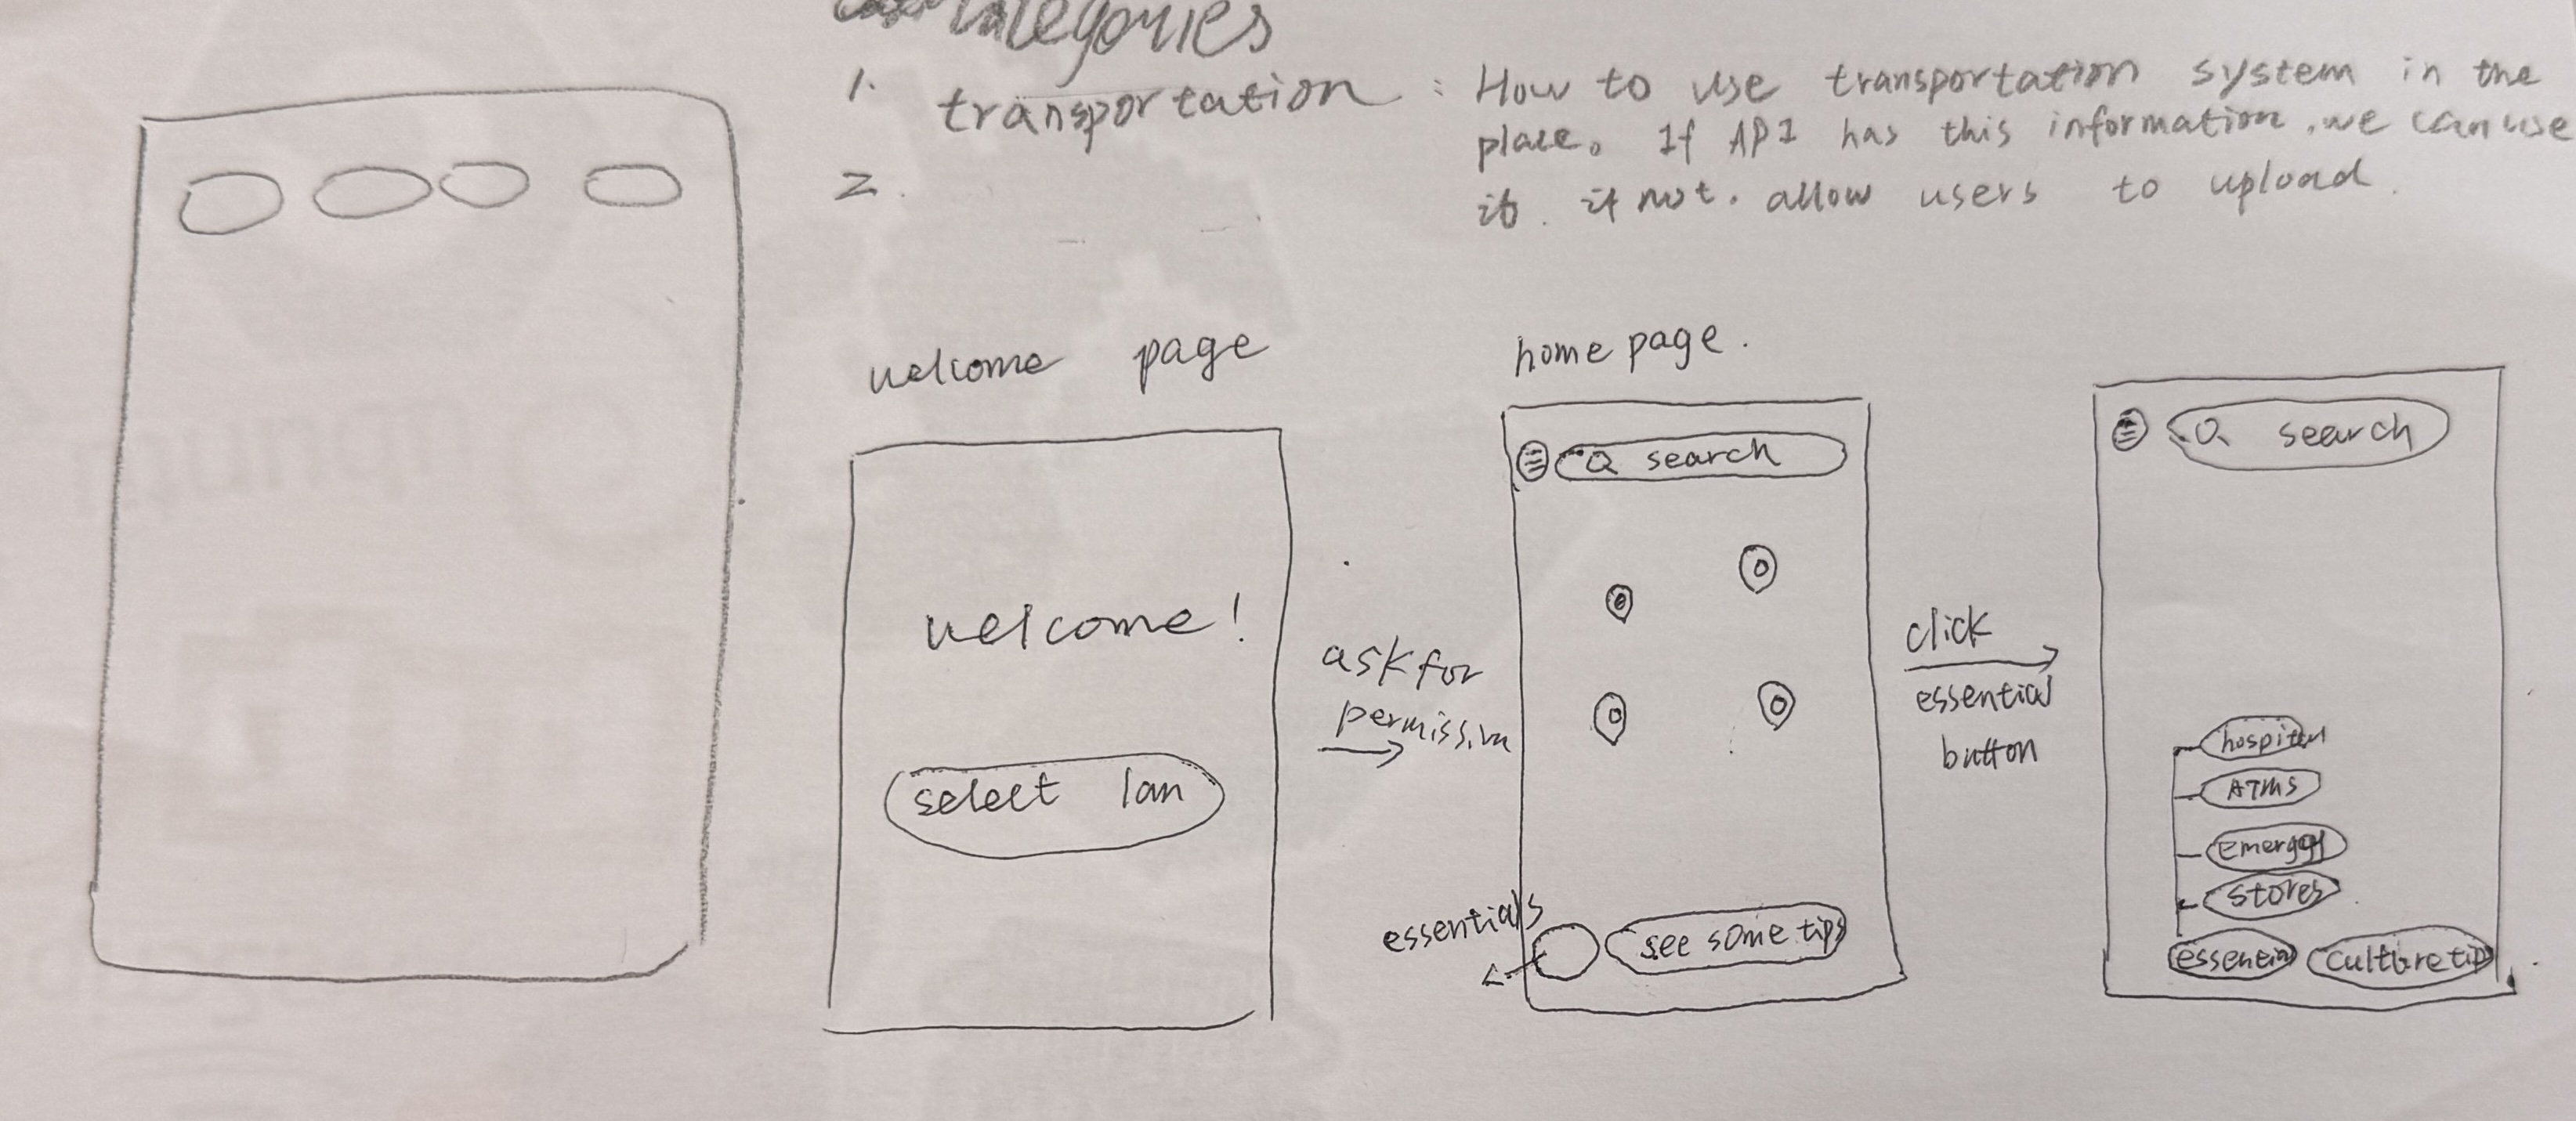
\includegraphics[height=0.3\textheight, keepaspectratio]{images/wireframing/firstHandDrawWirefame.jpg}
    \caption{Hand-Draw Wireframe Mobile View Version 1}
    \label{fig:appendix-wireframe-mobile-version-1}
\end{figure}

\begin{figure}[H]
    \centering
    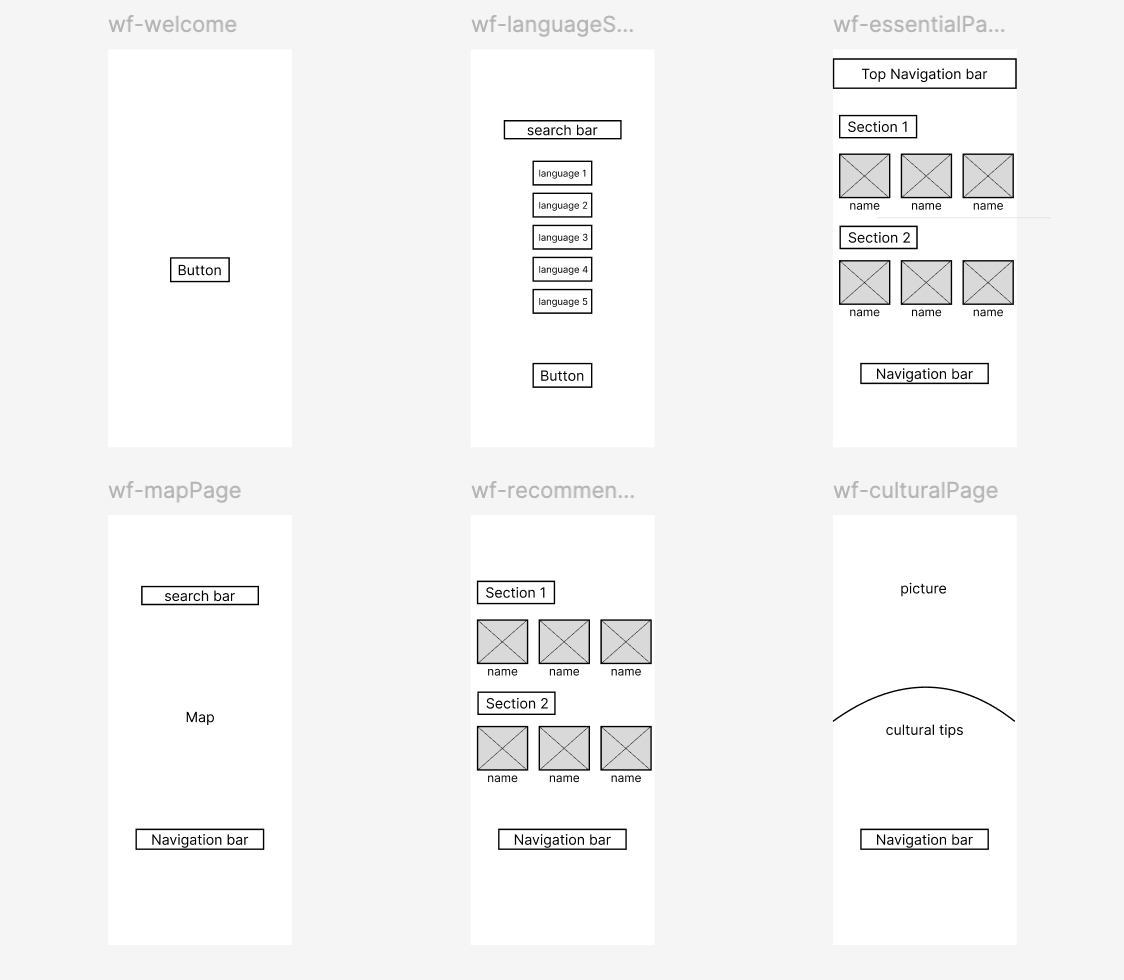
\includegraphics[height=0.3\textheight, keepaspectratio]{images/wireframing/mobileViewWireframing.png}
    \caption{Wireframe Mobile View Version 2}
    \label{fig:appendix-wireframe-mobile-version-2} 
\end{figure}

\begin{figure}[H]
    \centering
    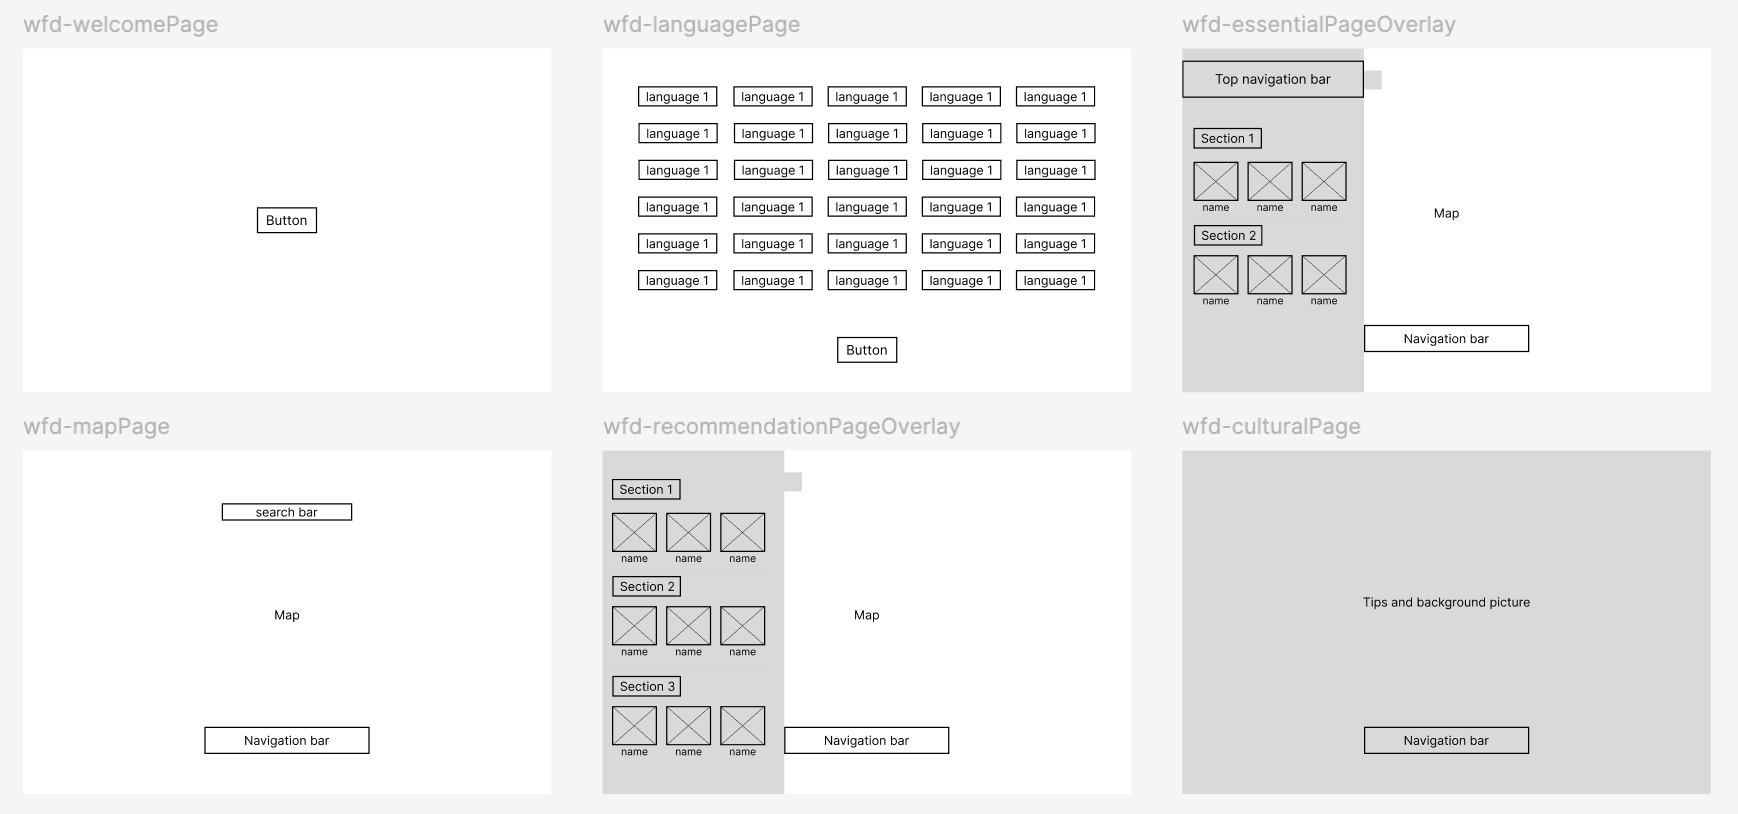
\includegraphics[height=0.3\textheight, keepaspectratio]{images/wireframing/desktopViewWireframing.png}
    \caption{Wireframe Desktop View}
    \label{fig:appendix-wireframe-desktop} 
\end{figure}

\section{Figma Prototypes}

\begin{figure}[H]
    \centering
    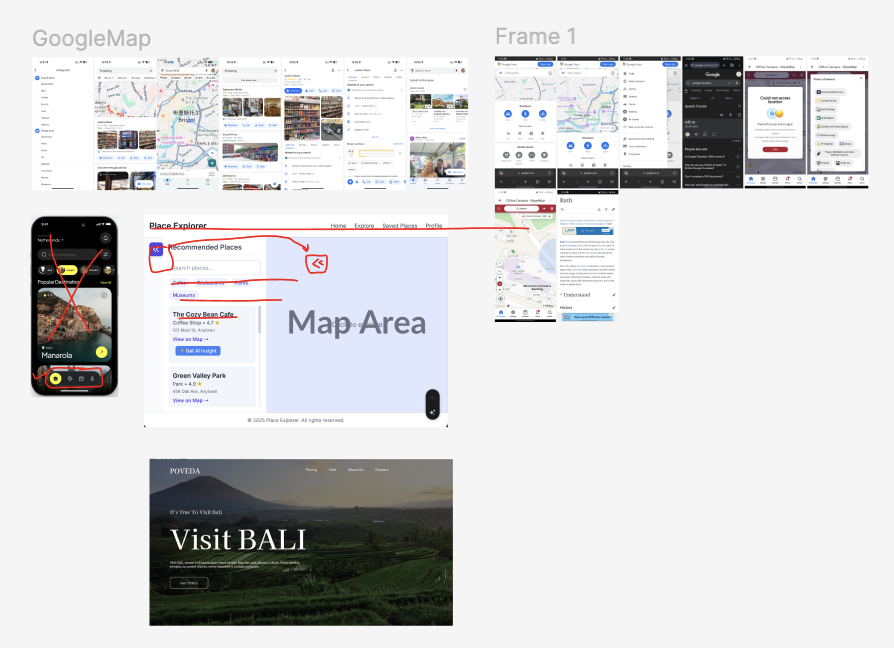
\includegraphics[height=0.3\textheight, keepaspectratio]{images/prototype/moodBoard.png}
    \caption{Prototype Inspiration Mood Board}
    \label{fig:appendix-mood-board}
\end{figure}

\begin{figure}[H]
    \centering
    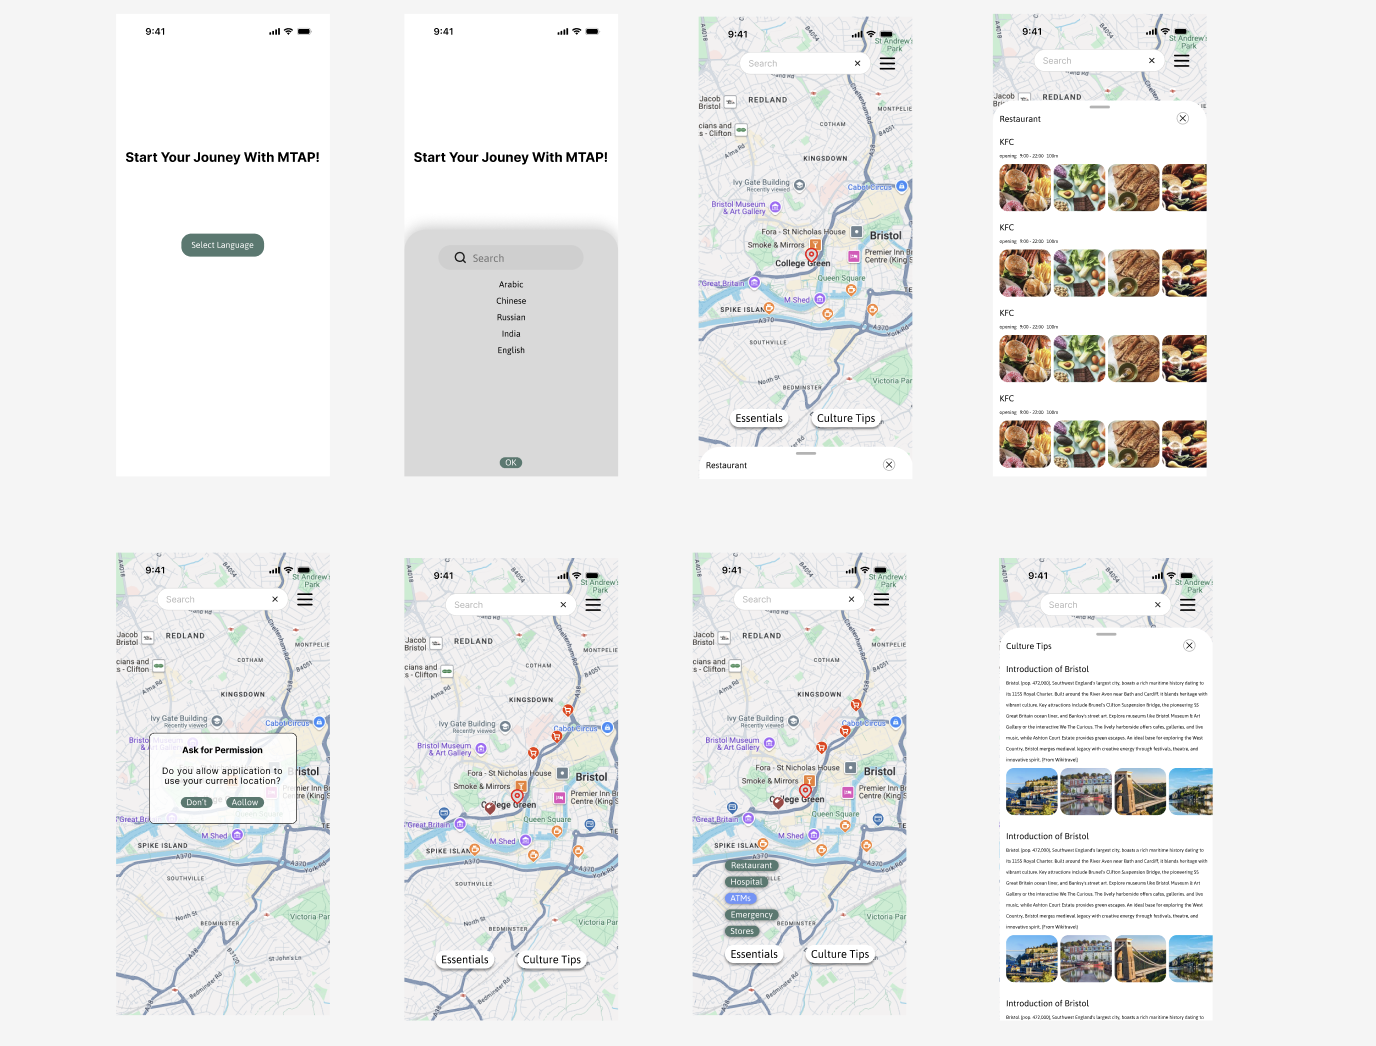
\includegraphics[height=0.3\textheight, keepaspectratio]{images/prototype/mobilePrototypeVersion1.png}
    \caption{Prototype Mobile View Before Initial Evaluation}
    \label{fig:appendix-prototype-mobile1} 
\end{figure}

\begin{figure}[H]
    \centering
    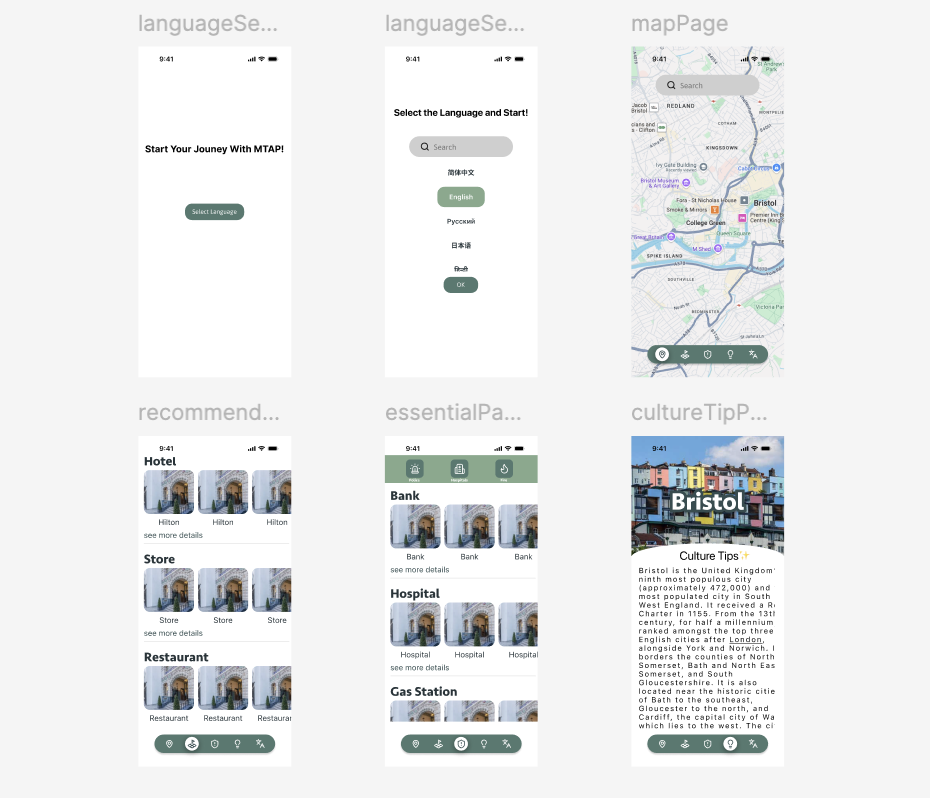
\includegraphics[height=0.3\textheight, keepaspectratio]{images/prototype/mobilePrototypeVersion2.png}
    \caption{Prototype Mobile View After Initial Evaluation}
    \label{fig:appendix-prototype-mobile2} 
\end{figure}

\begin{figure}[H]
    \centering
    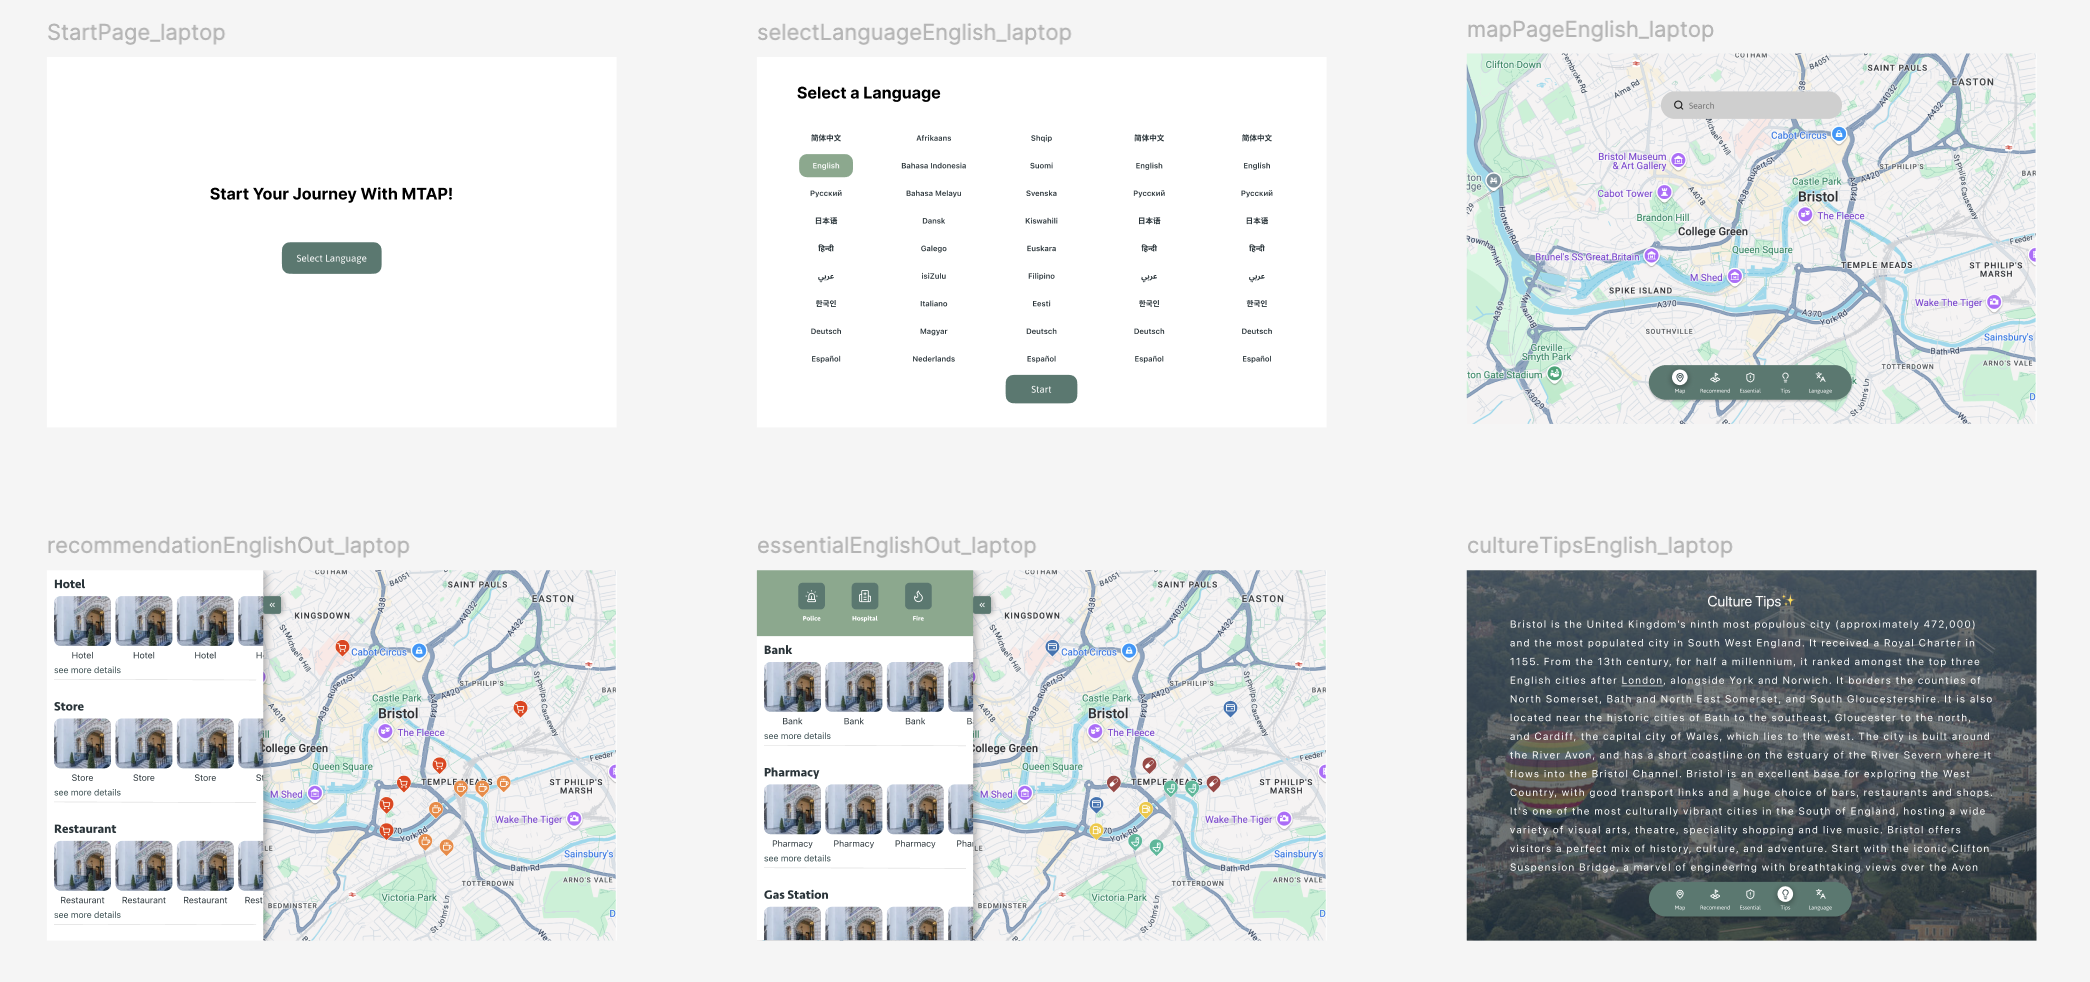
\includegraphics[height=0.3\textheight, keepaspectratio]{images/prototype/desktopPrototype.png}
    \caption{Prototype Desktop View}
    \label{fig:appendix-prototype-desktop} 
\end{figure}

\section{Guide Screen}
\begin{figure}[H]
    \centering
    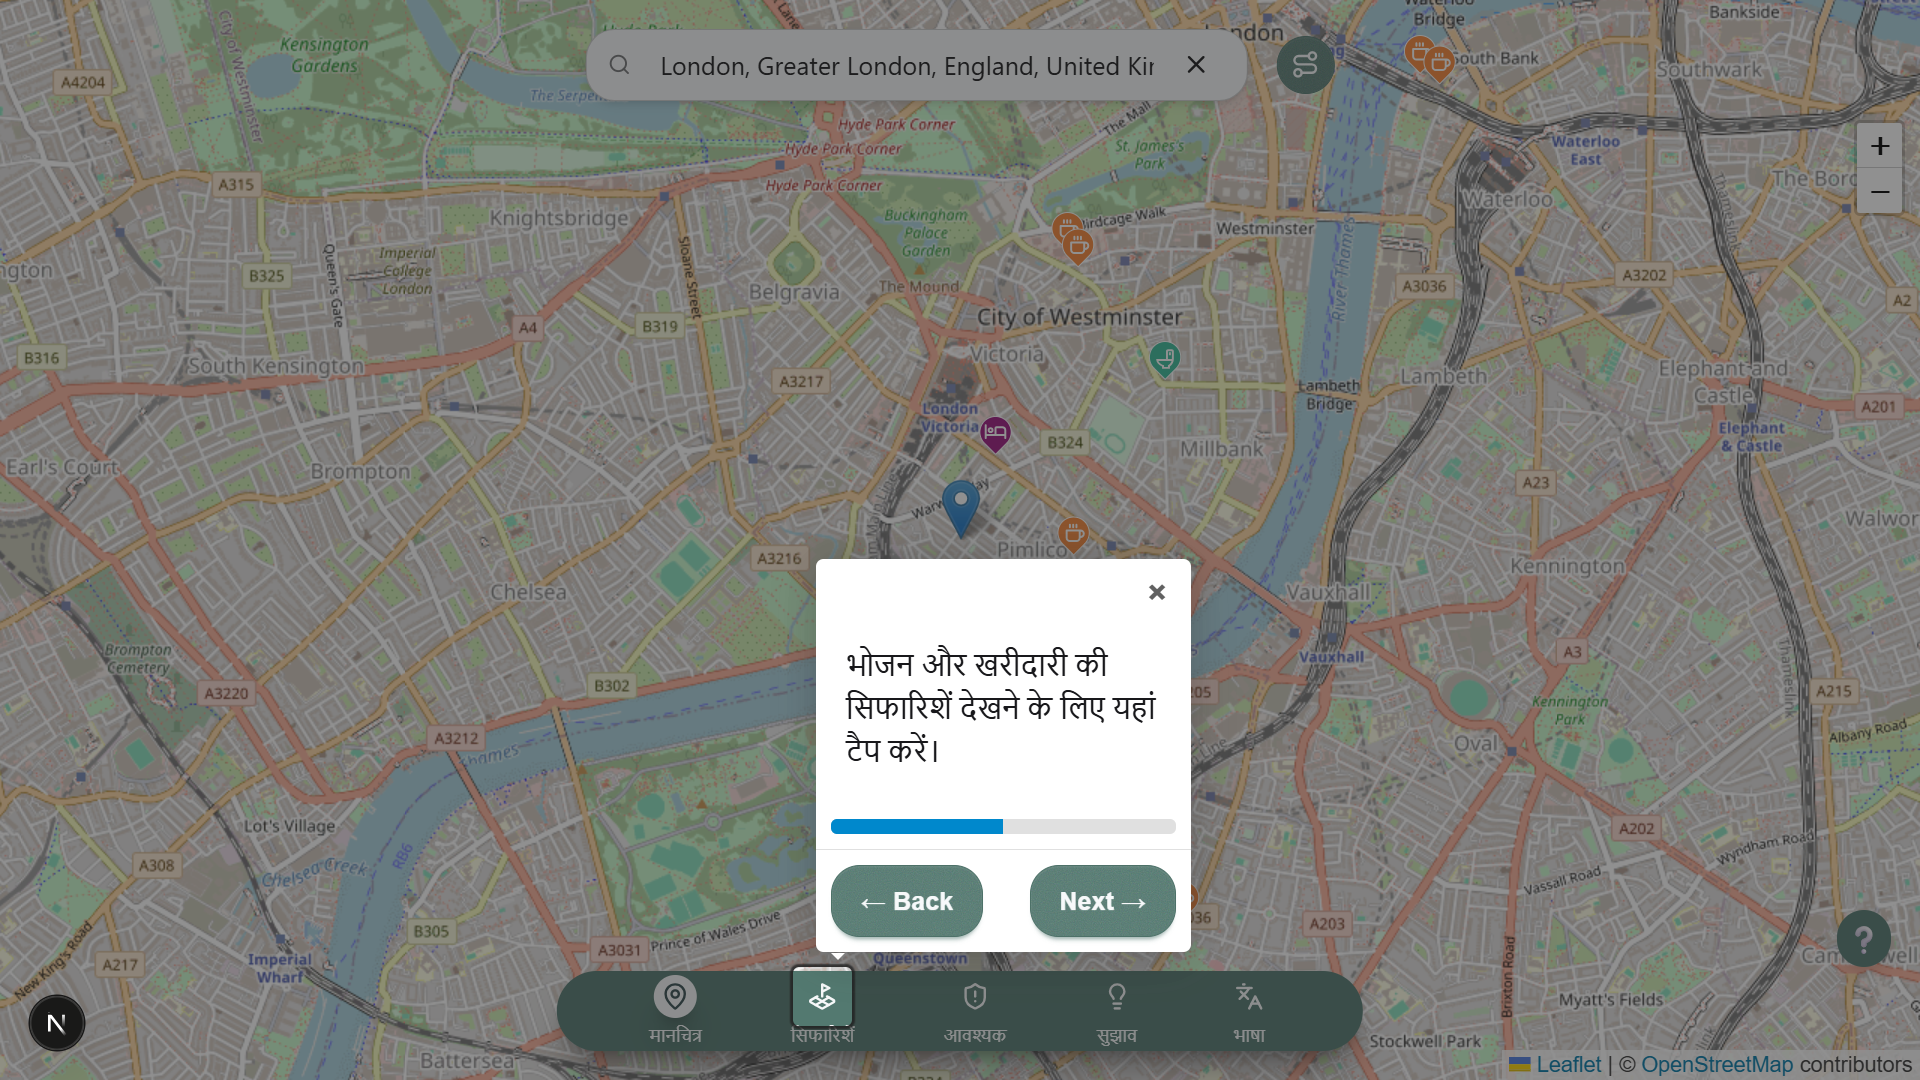
\includegraphics[height=0.2\textheight,keepaspectratio]{images/Screenshots/0_guide_desktop.png}
    \caption{Guide screen (Desktop)}
    \label{fig:Guide-screen-(Desktop}
\end{figure}

\begin{figure}[H]
    \centering
    \includegraphics[height=0.2\textheight,keepaspectratio]{images/Screenshots/0_guide_mobile.png}
    \caption{Guide screen (Mobile)}
\end{figure}

\section{Language Screen}
\begin{figure}[H]
    \centering
    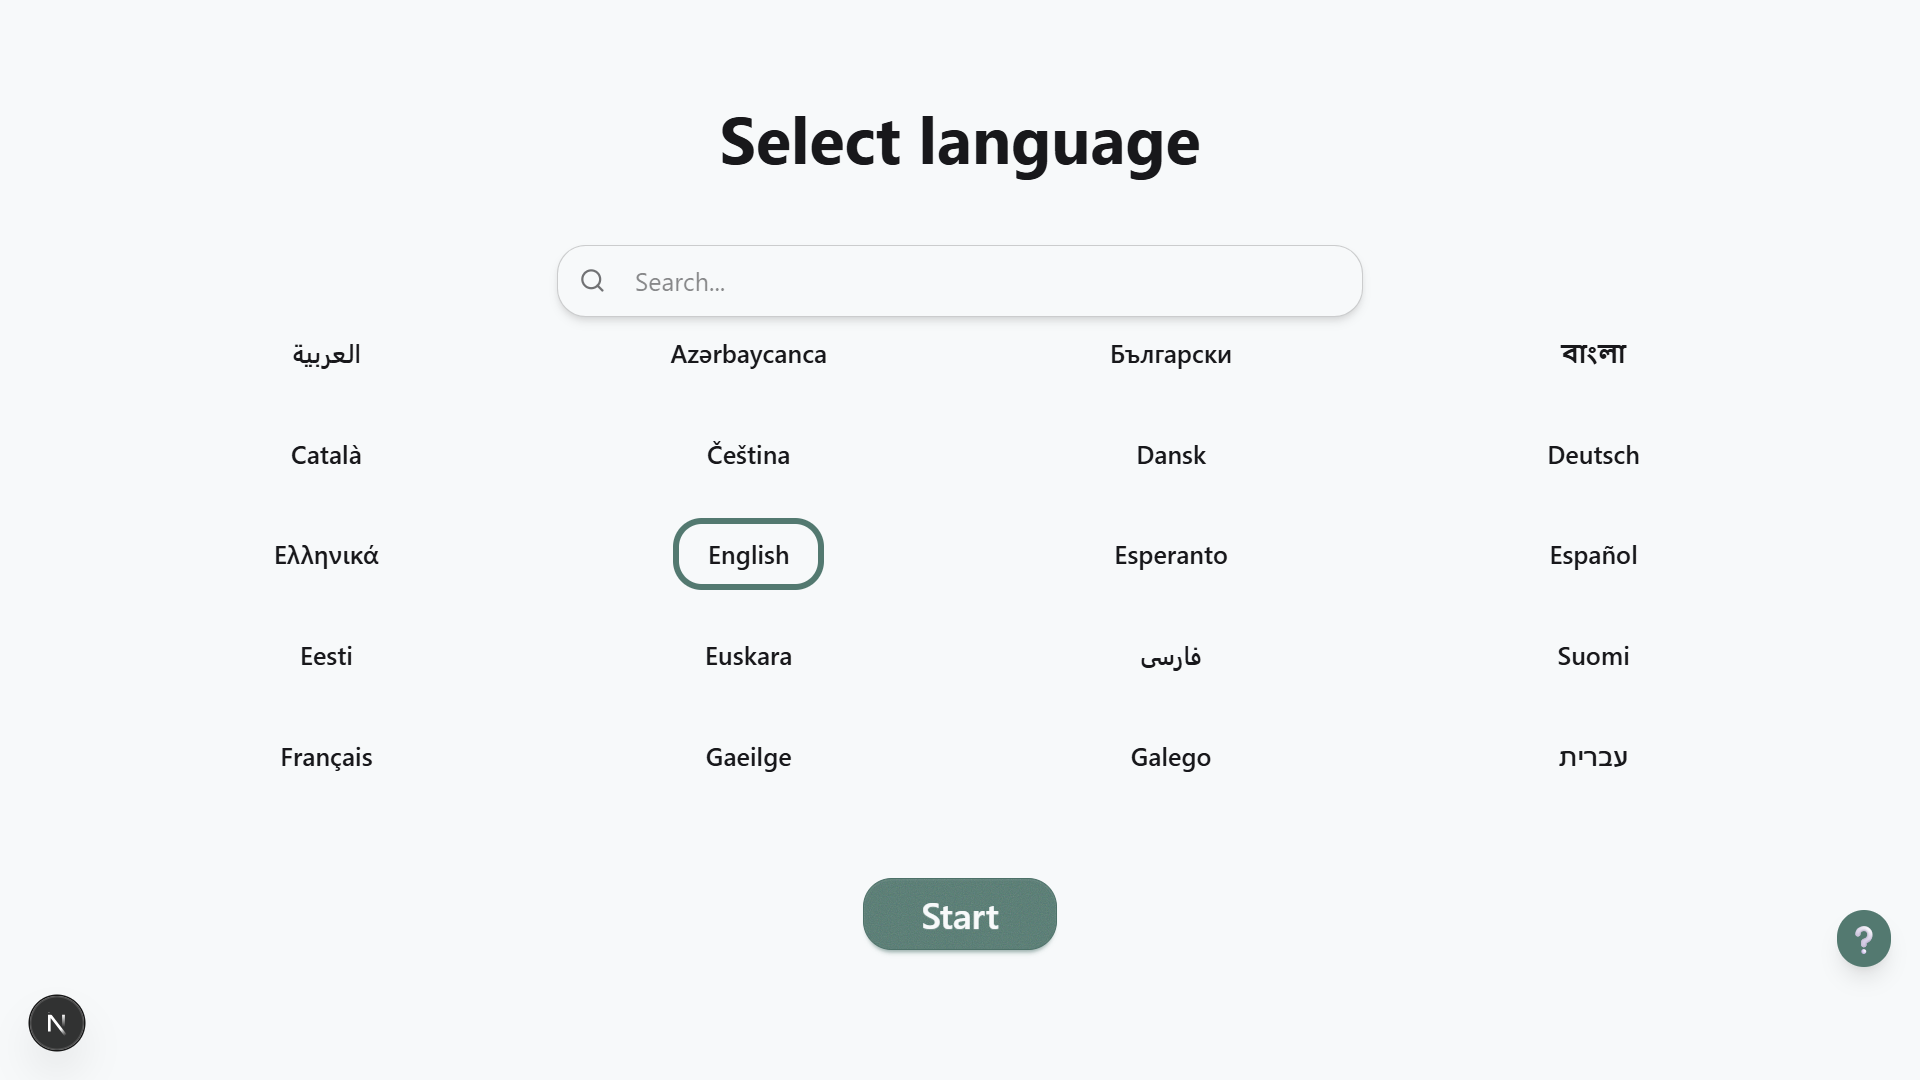
\includegraphics[height=0.3\textheight,keepaspectratio]{images/Screenshots/1_language_desktop.png}
    \caption{Language screen (Desktop)}
\end{figure}

\begin{figure}[H]
    \centering
    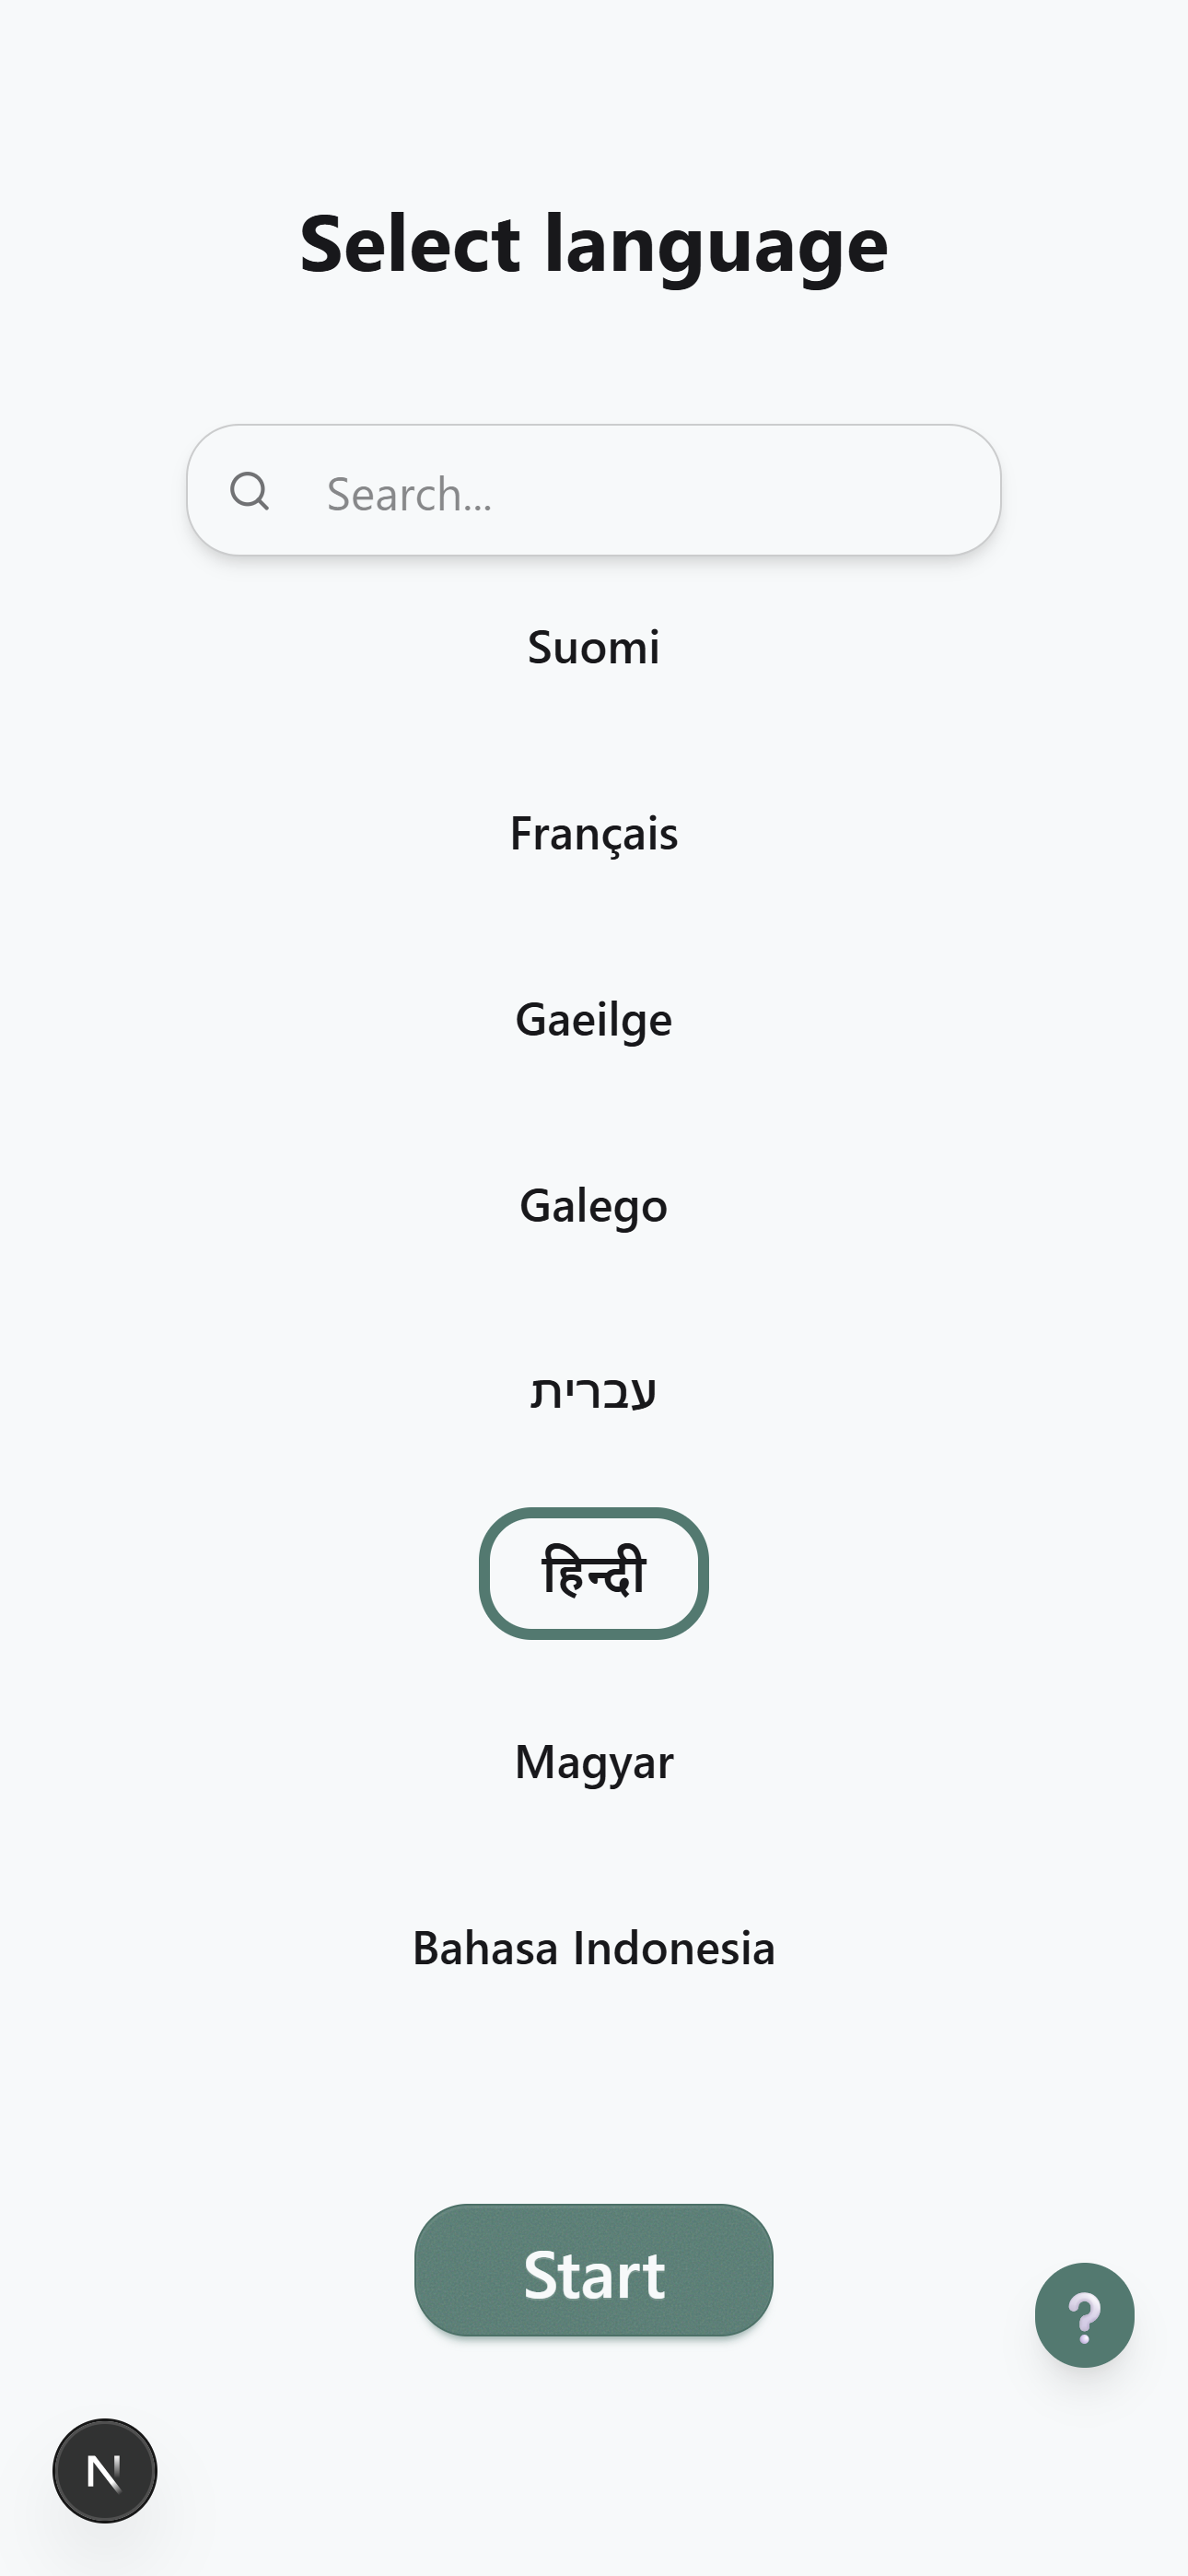
\includegraphics[height=0.3\textheight,keepaspectratio]{images/Screenshots/1_language_mobile.png}
    \caption{Language screen (Mobile)}
\end{figure}

\section{Map Screen}
\begin{figure}[H]
    \centering
    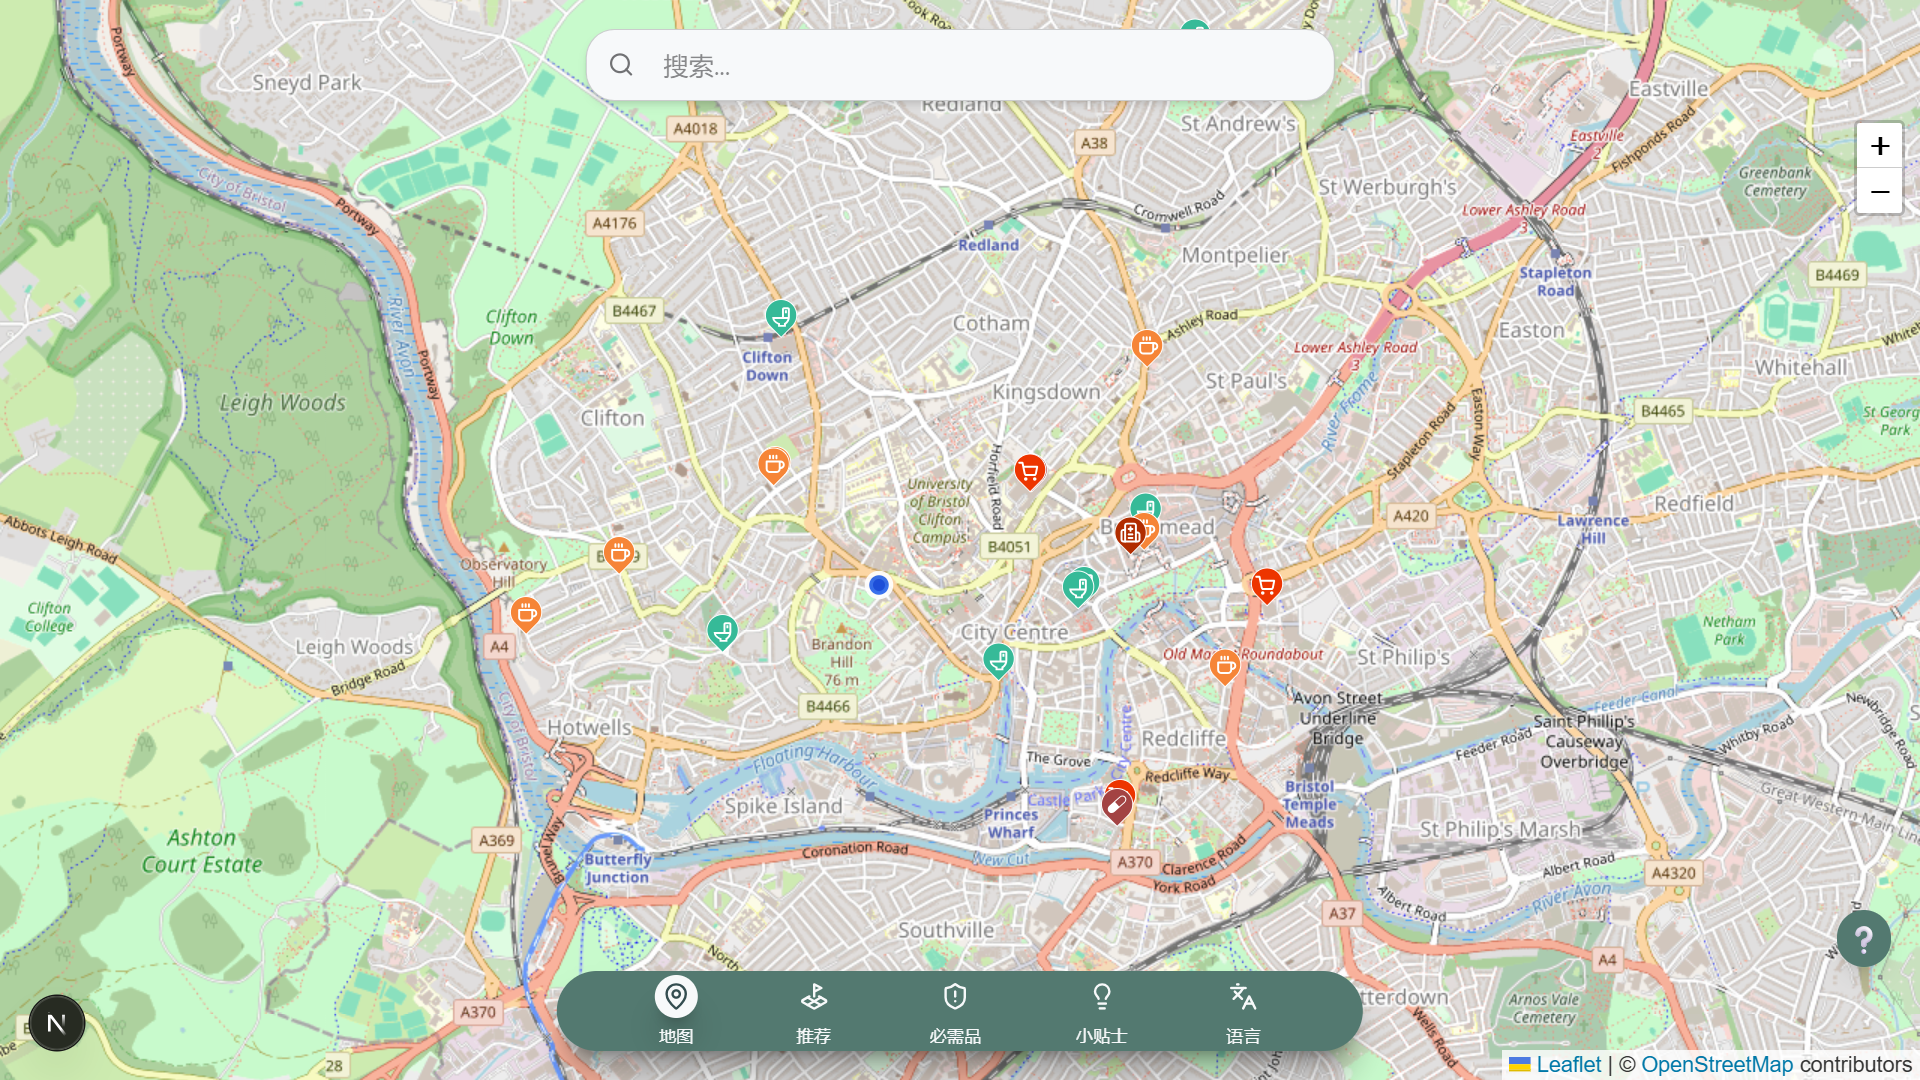
\includegraphics[height=0.3\textheight,keepaspectratio]{images/Screenshots/2_map_desktop.png}
    \caption{Map screen (Desktop)}
\end{figure}

\begin{figure}[H]
    \centering
    \includegraphics[height=0.3\textheight,keepaspectratio]{images/Screenshots/2_map_mobile.png}
    \caption{Map screen (Mobile)}
\end{figure}

\section{Side Panel Screen}
\begin{figure}[H]
    \centering
    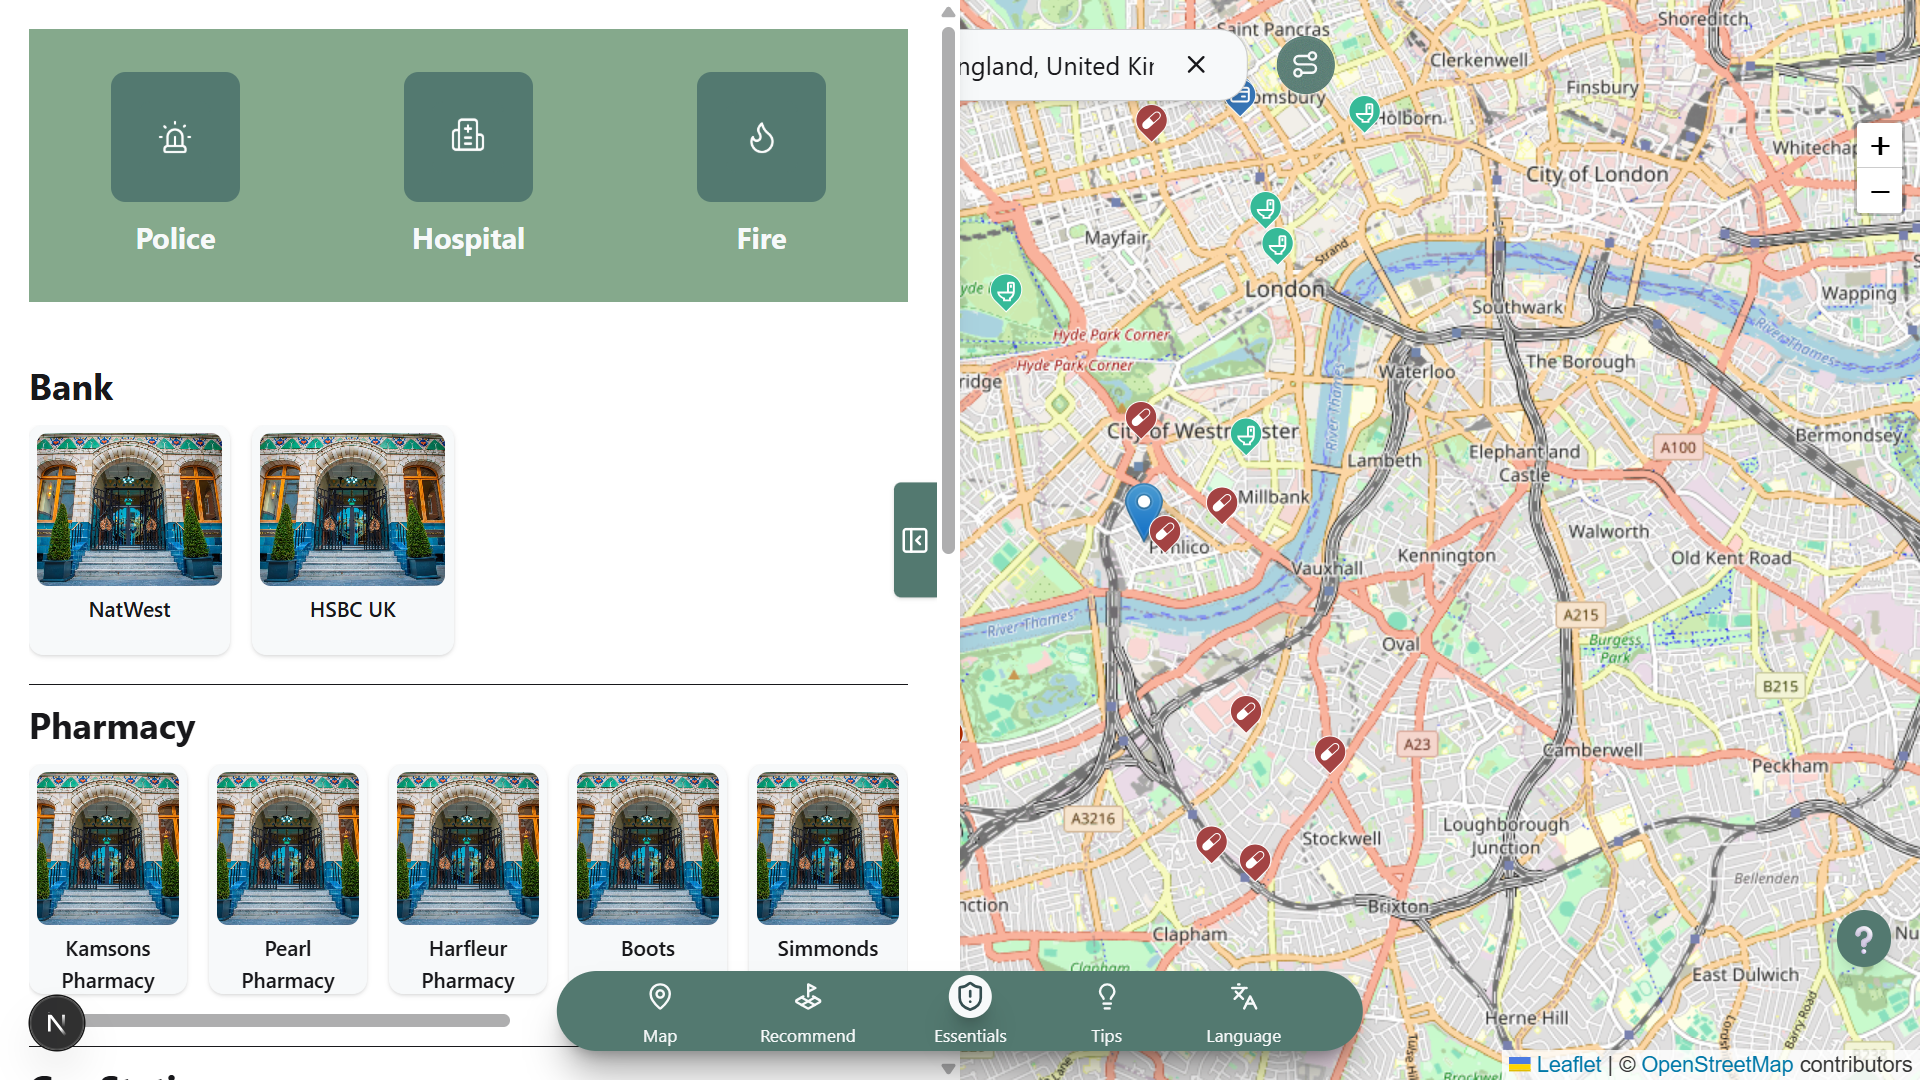
\includegraphics[height=0.3\textheight,keepaspectratio]{images/Screenshots/3_sidepanel_desktop.png}
    \caption{Side Panel screen (Desktop)}
    \label{fig:Side-Panel-screen-(Desktop)}
\end{figure}

\begin{figure}[H]
    \centering
    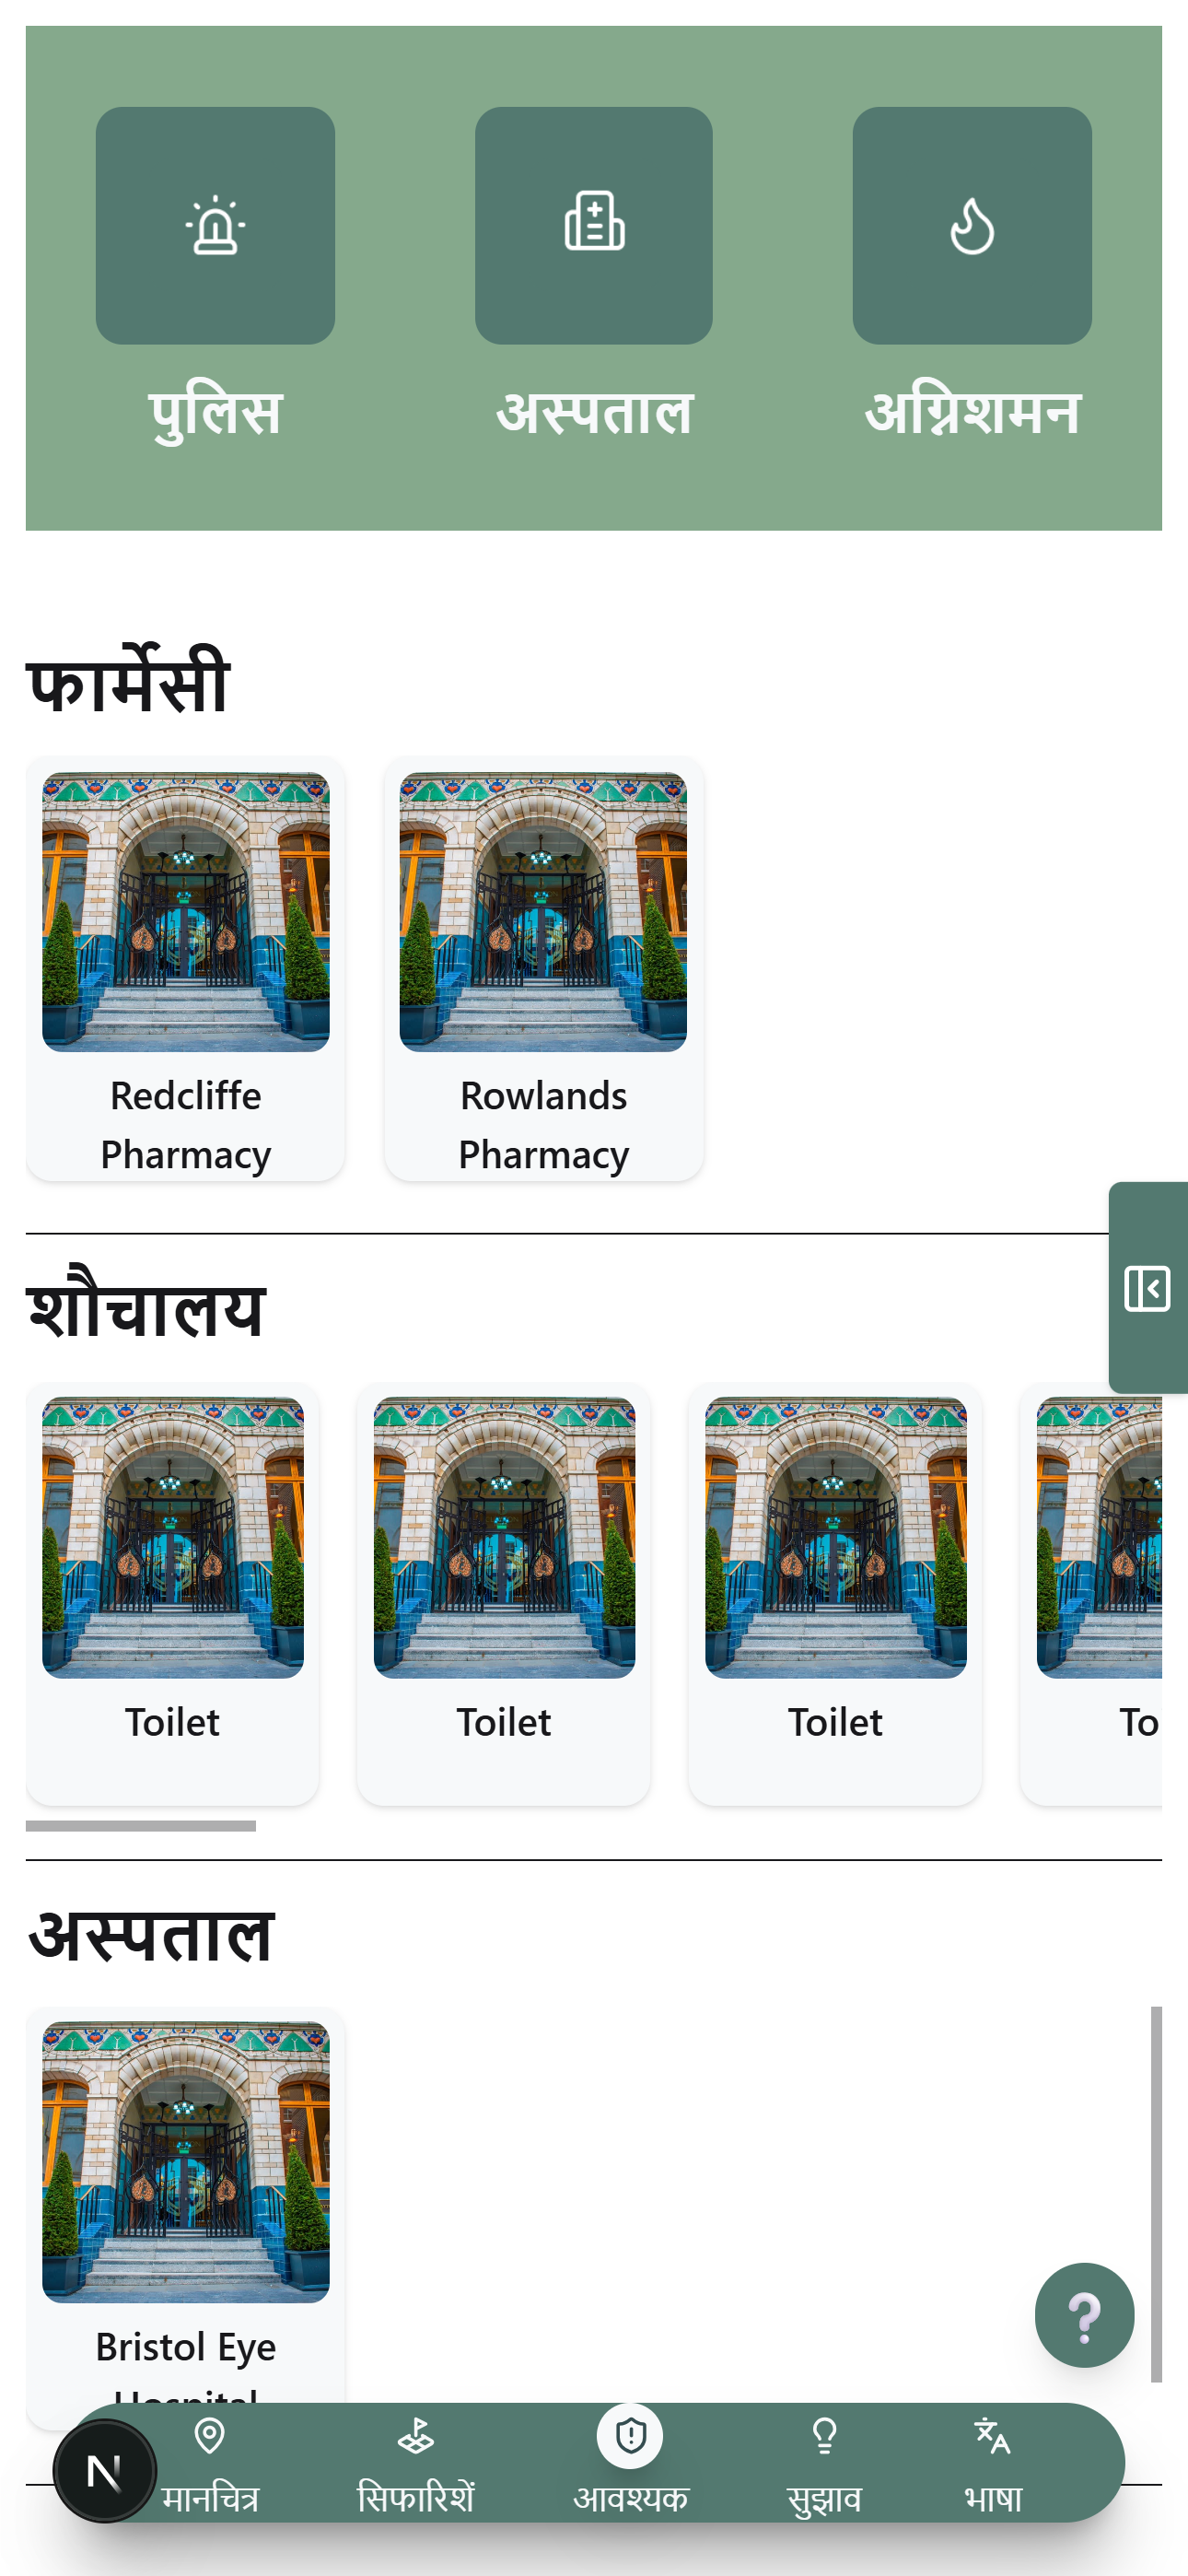
\includegraphics[height=0.3\textheight,keepaspectratio]{images/Screenshots/3_sidepanel_mobile.png}
    \caption{Side Panel screen (Mobile)}
    \label{fig:Side-Panel-screen-(Mobile)}
\end{figure}

\section{Directions Screen}
\begin{figure}[H]
    \centering
    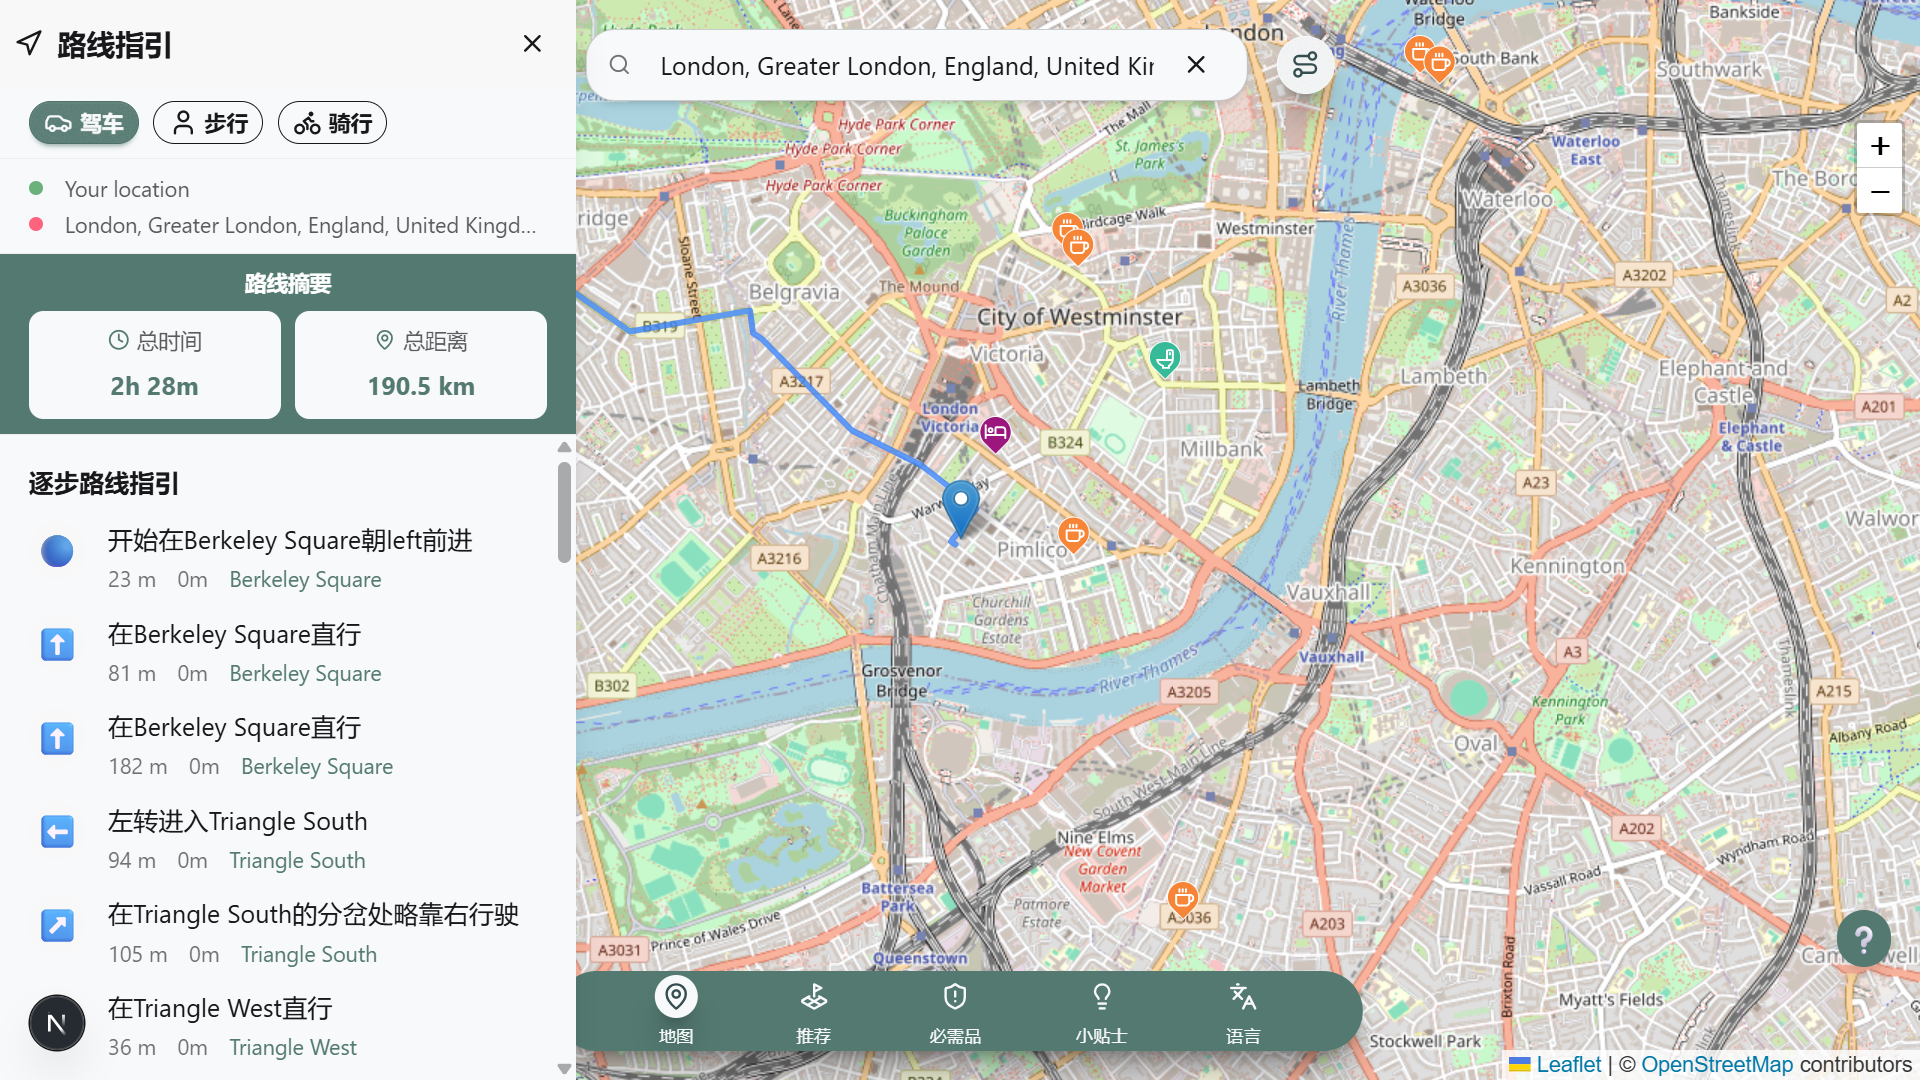
\includegraphics[height=0.3\textheight,keepaspectratio]{images/Screenshots/4_directions_desktop.png}
    \caption{Directions screen (Desktop)}
\end{figure}

\begin{figure}[H]
    \centering
    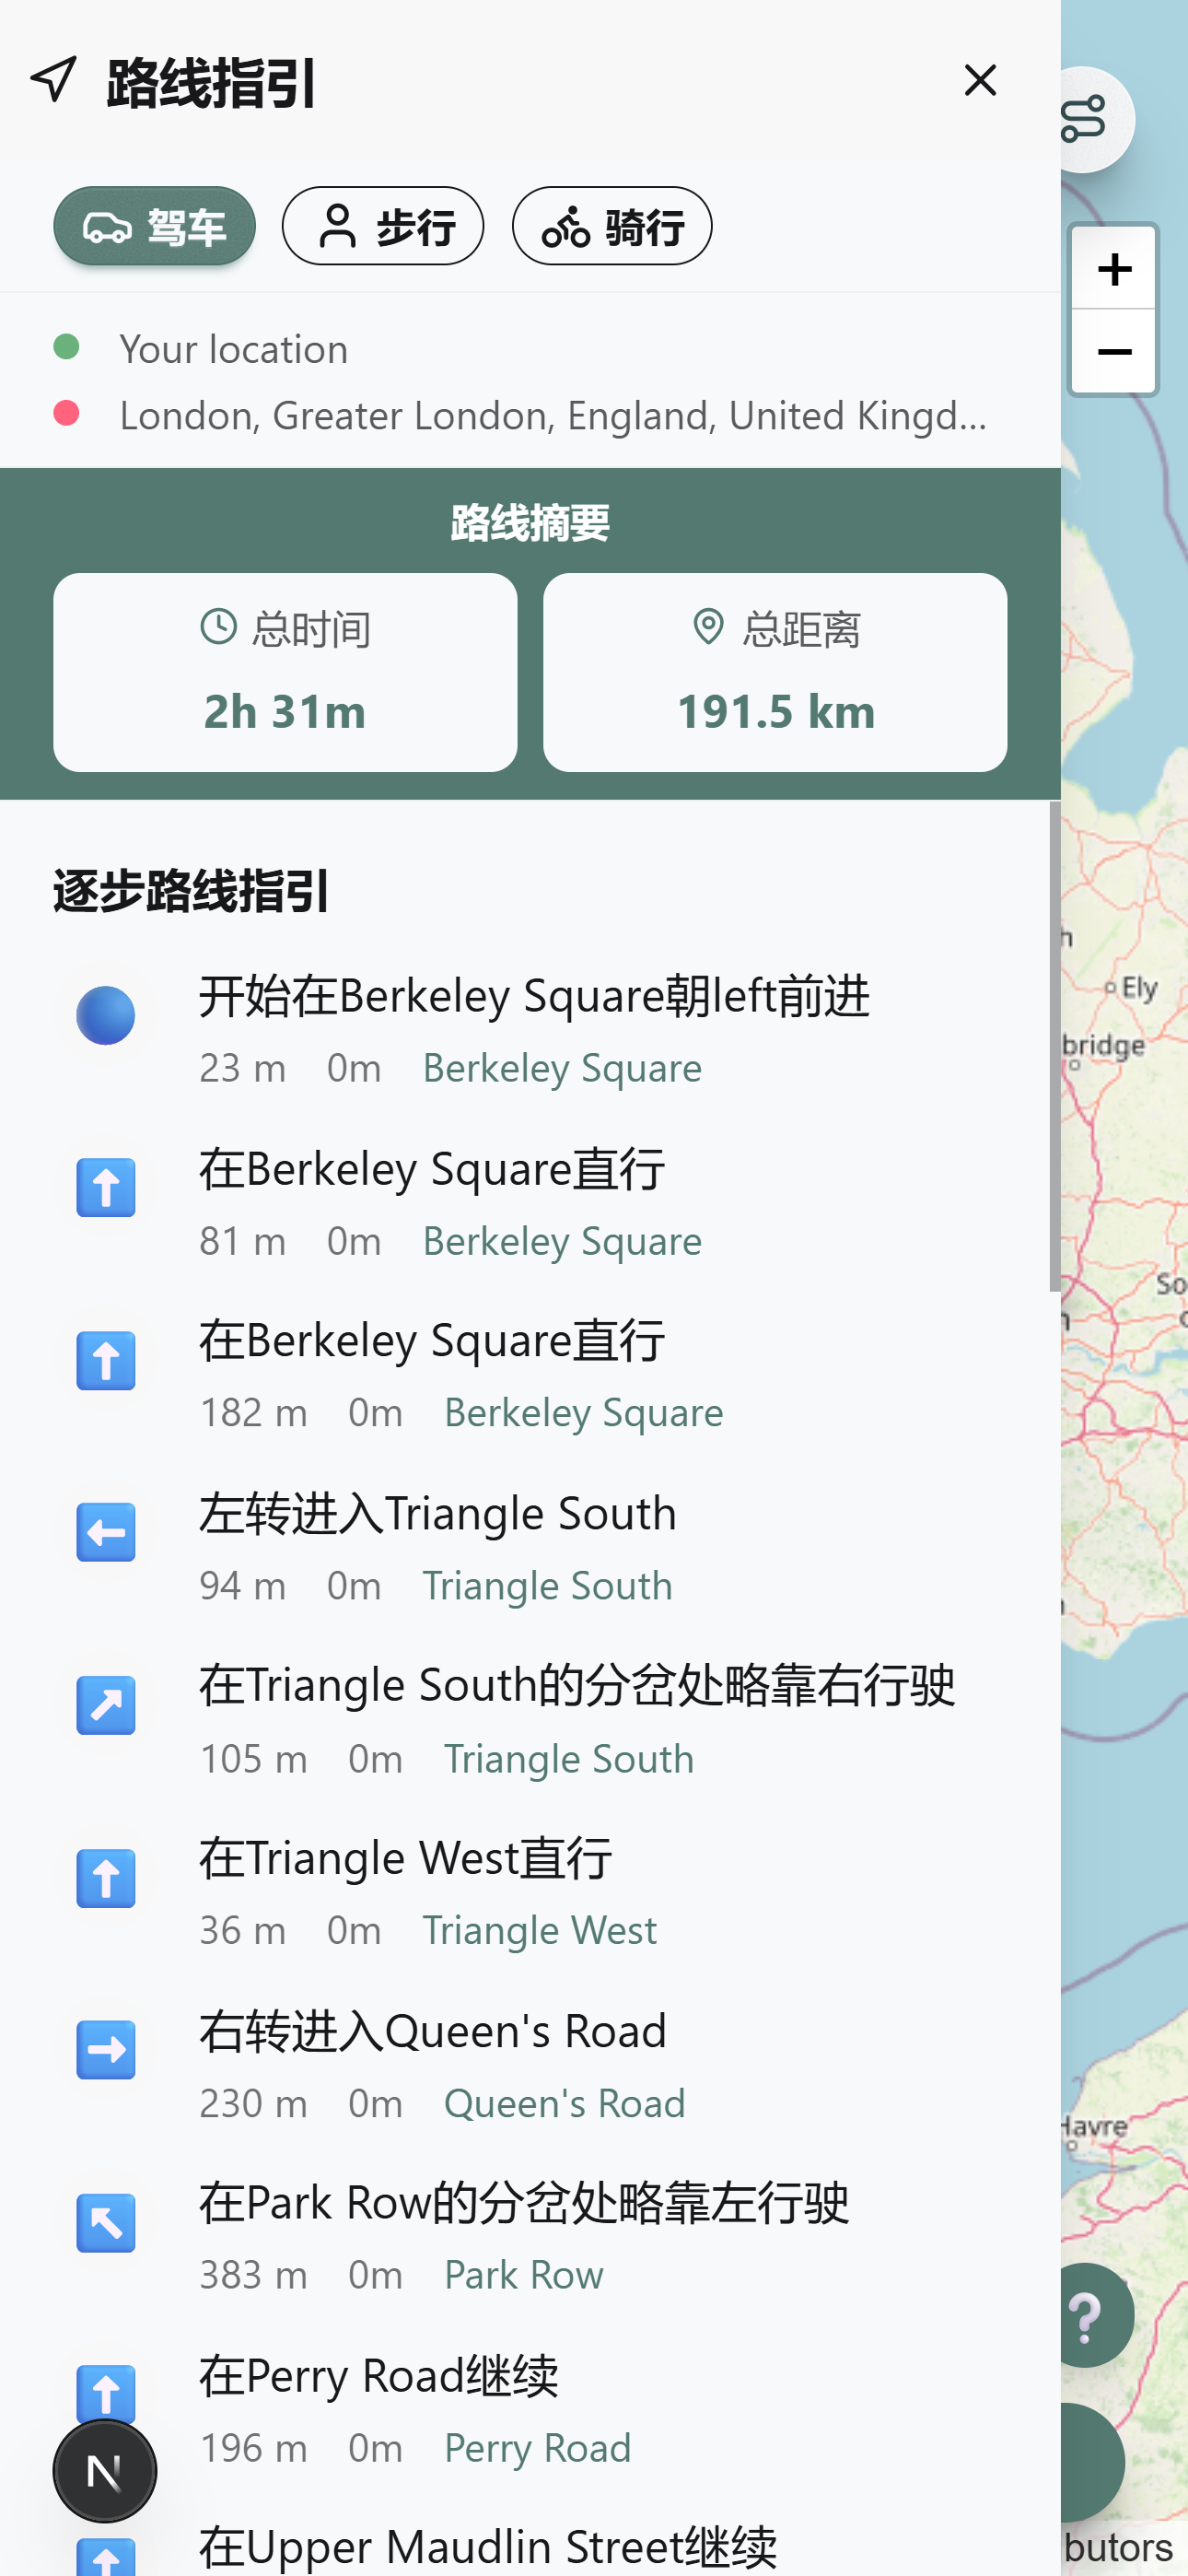
\includegraphics[height=0.3\textheight,keepaspectratio]{images/Screenshots/4_directions_mobile.png}
    \caption{Directions screen (Mobile)}
\end{figure}

\section{Cultural Tips Screen}
\begin{figure}[H]
    \centering
    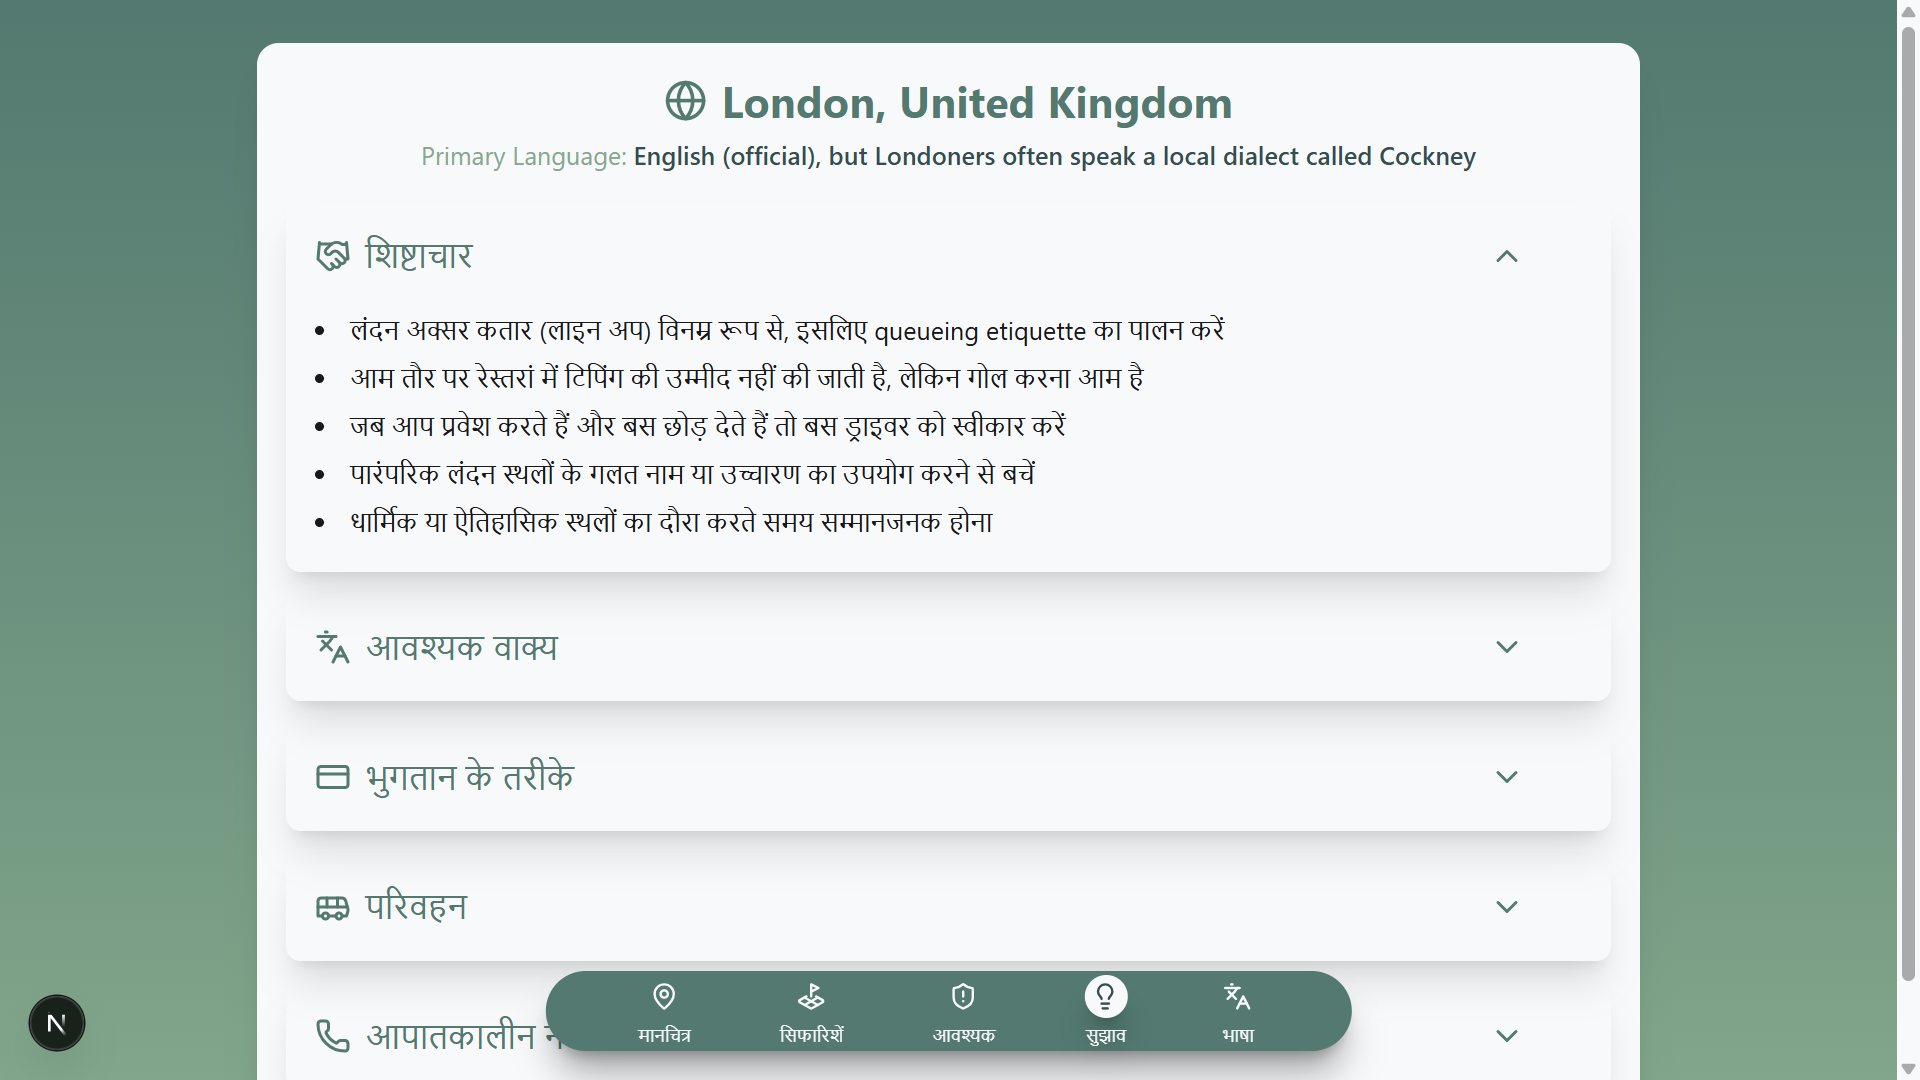
\includegraphics[height=0.3\textheight,keepaspectratio]{images/Screenshots/5_culturaltips_desktop.png}
    \caption{Cultural Tips screen (Desktop)}
\end{figure}

\begin{figure}[H]
    \centering
    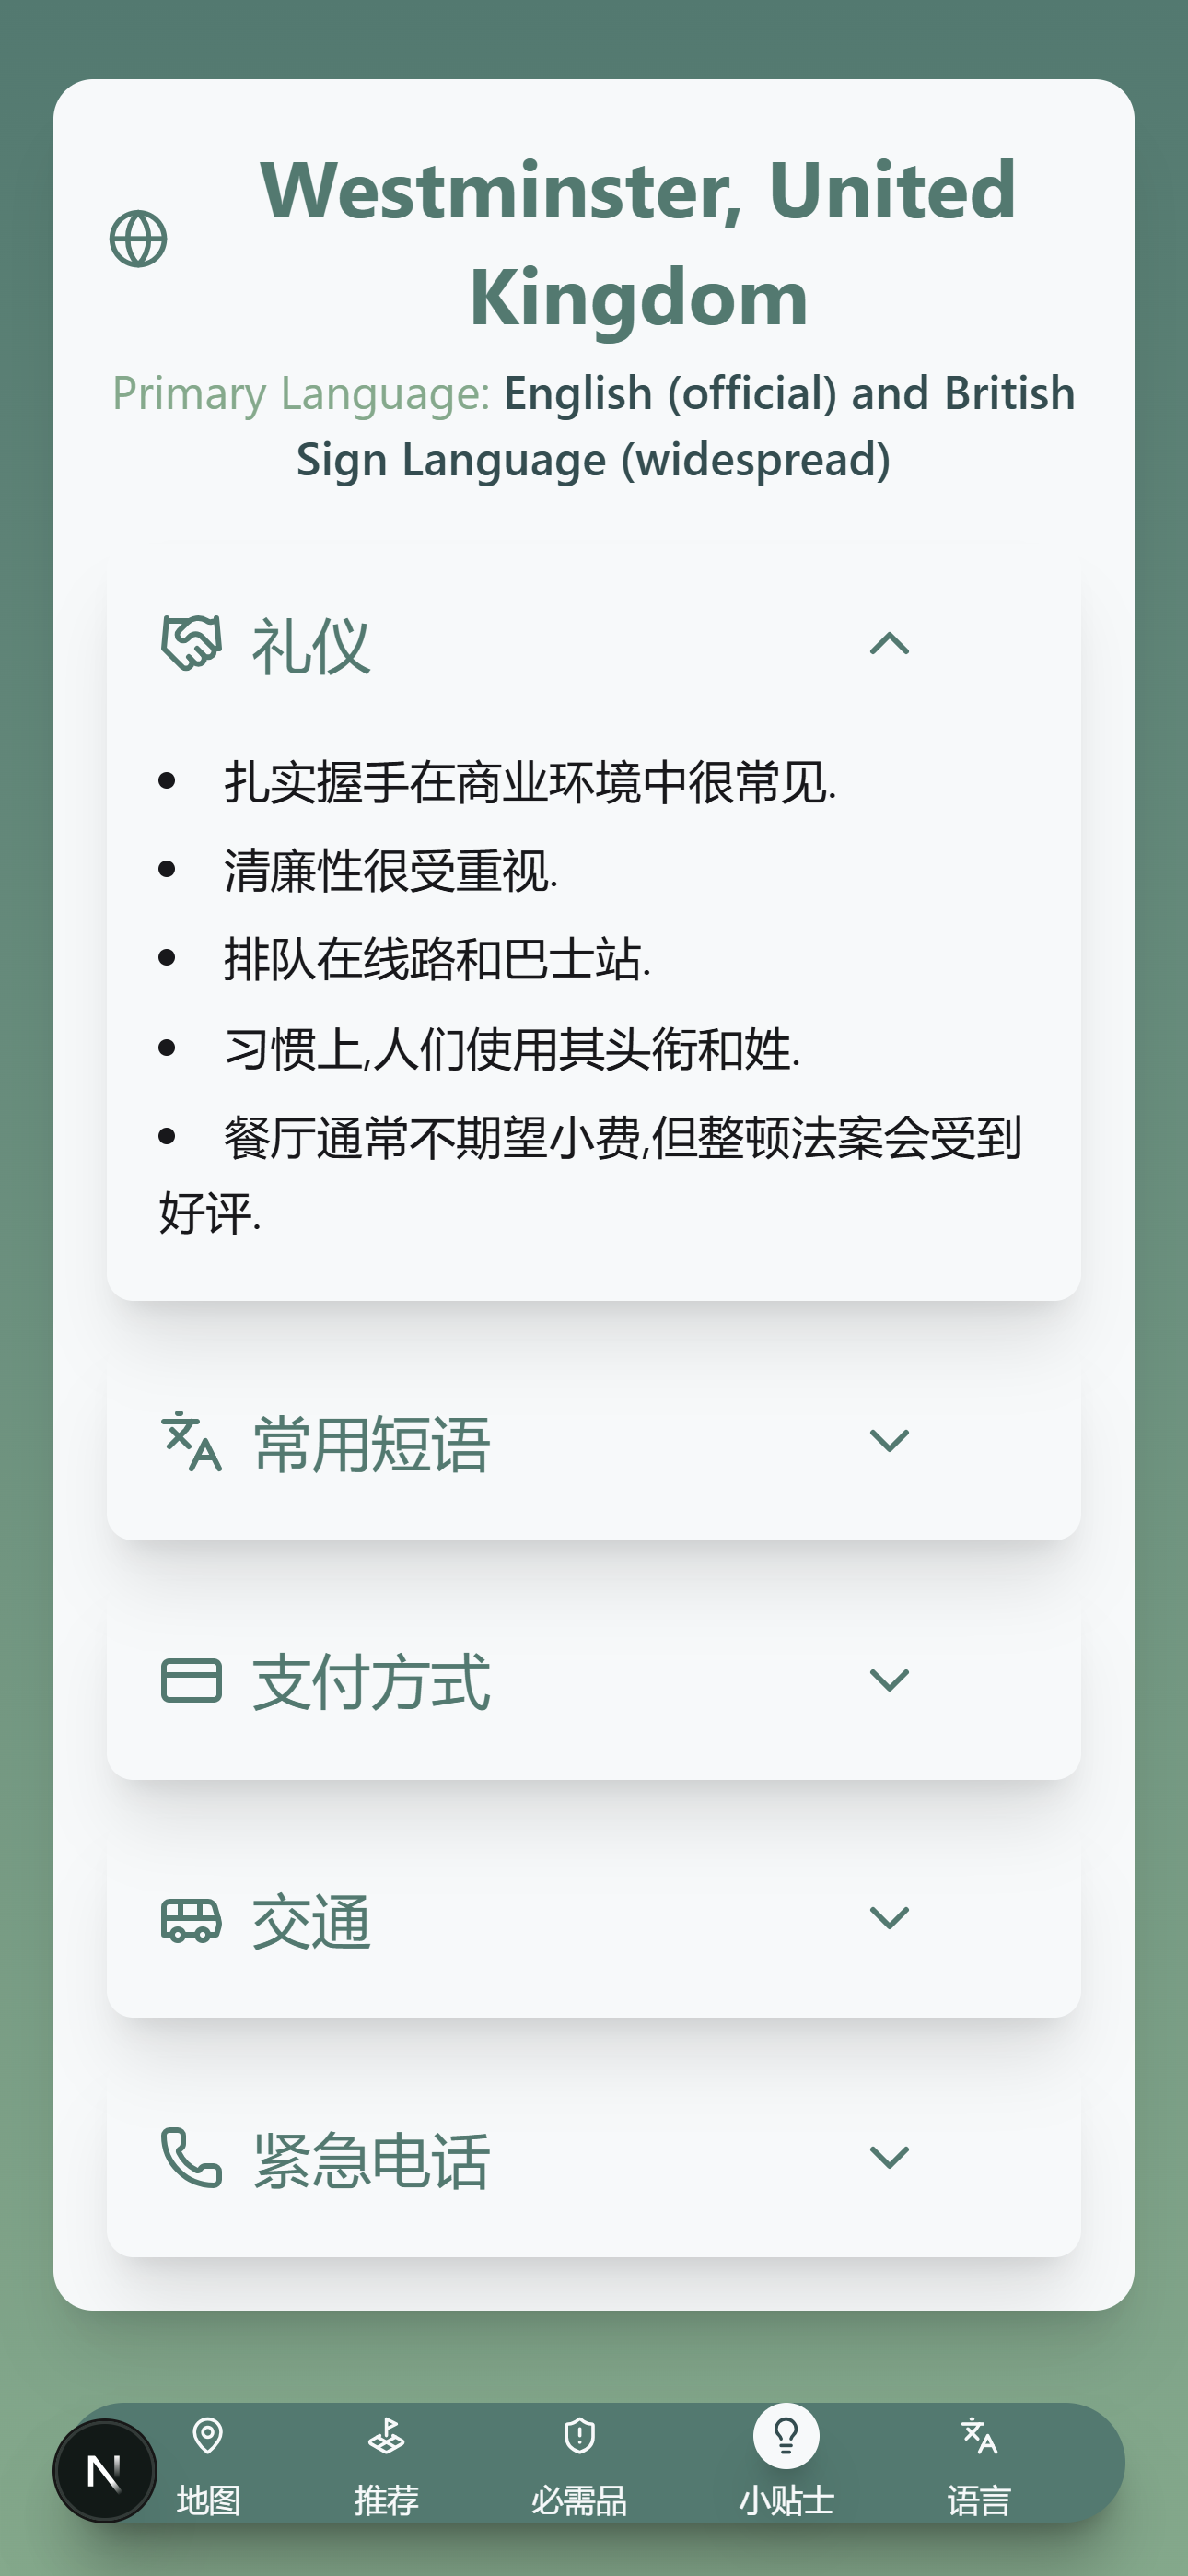
\includegraphics[height=0.3\textheight,keepaspectratio]{images/Screenshots/5_culturaltips_mobile.png}
    \caption{Cultural Tips screen (Mobile)}
\end{figure}

%%%%%%%%%%%%%%%%%%%%%% Postman Results %%%%%%%%%%%
\section{Postman Results}
\begin{figure}[H]
    \centering
    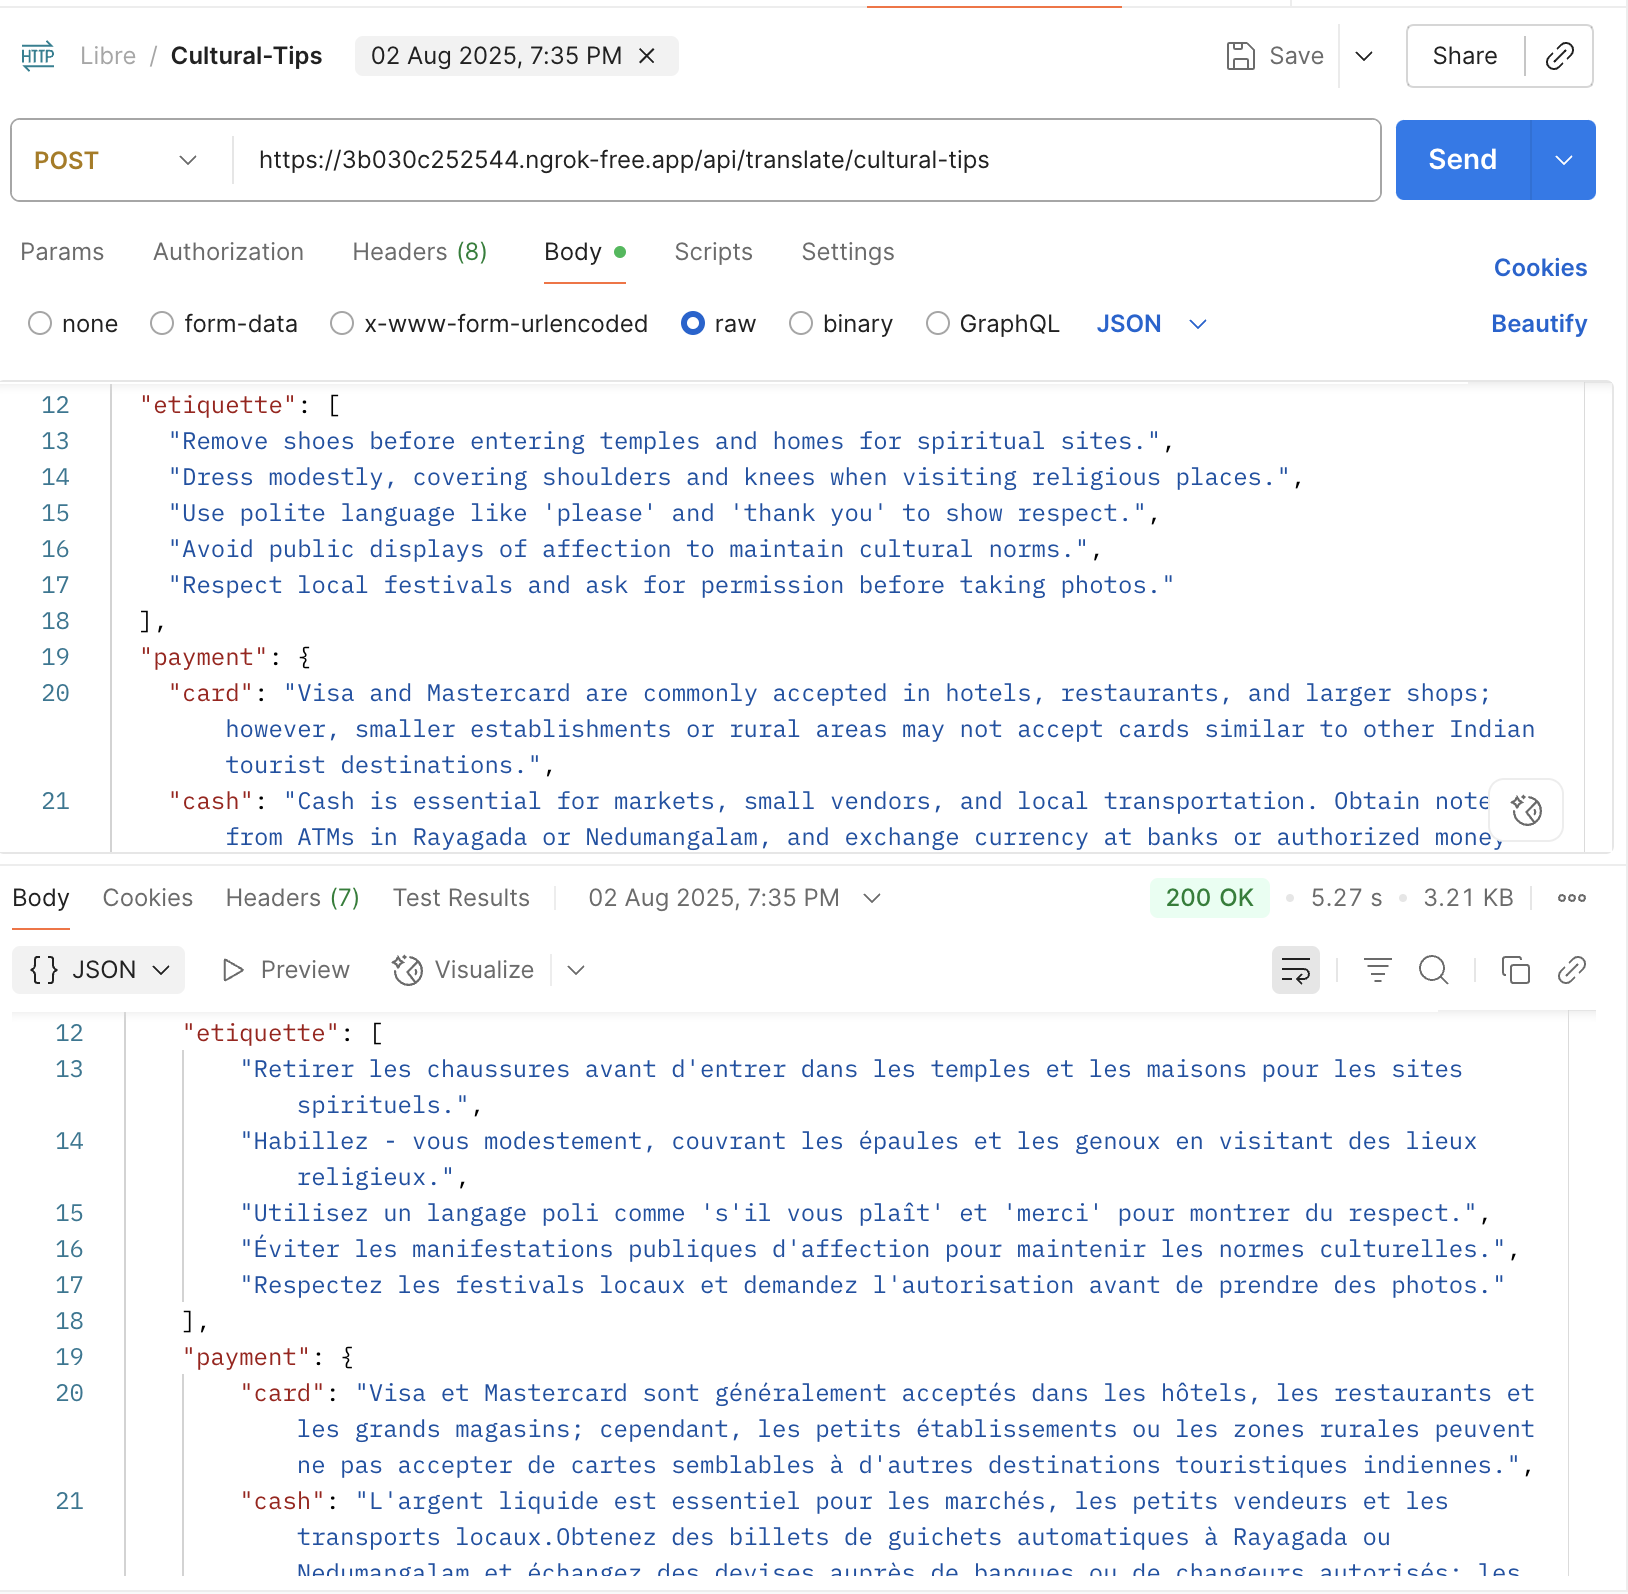
\includegraphics[width=1\linewidth]{images/Backend/Translation_Service_first_iteration.png}
    \caption{The image shows initial response time for translation of cultural tips data to be 5.27 seconds.}
    \label{fig:intial_response_time}
\end{figure}

\begin{figure}[H]
    \centering
    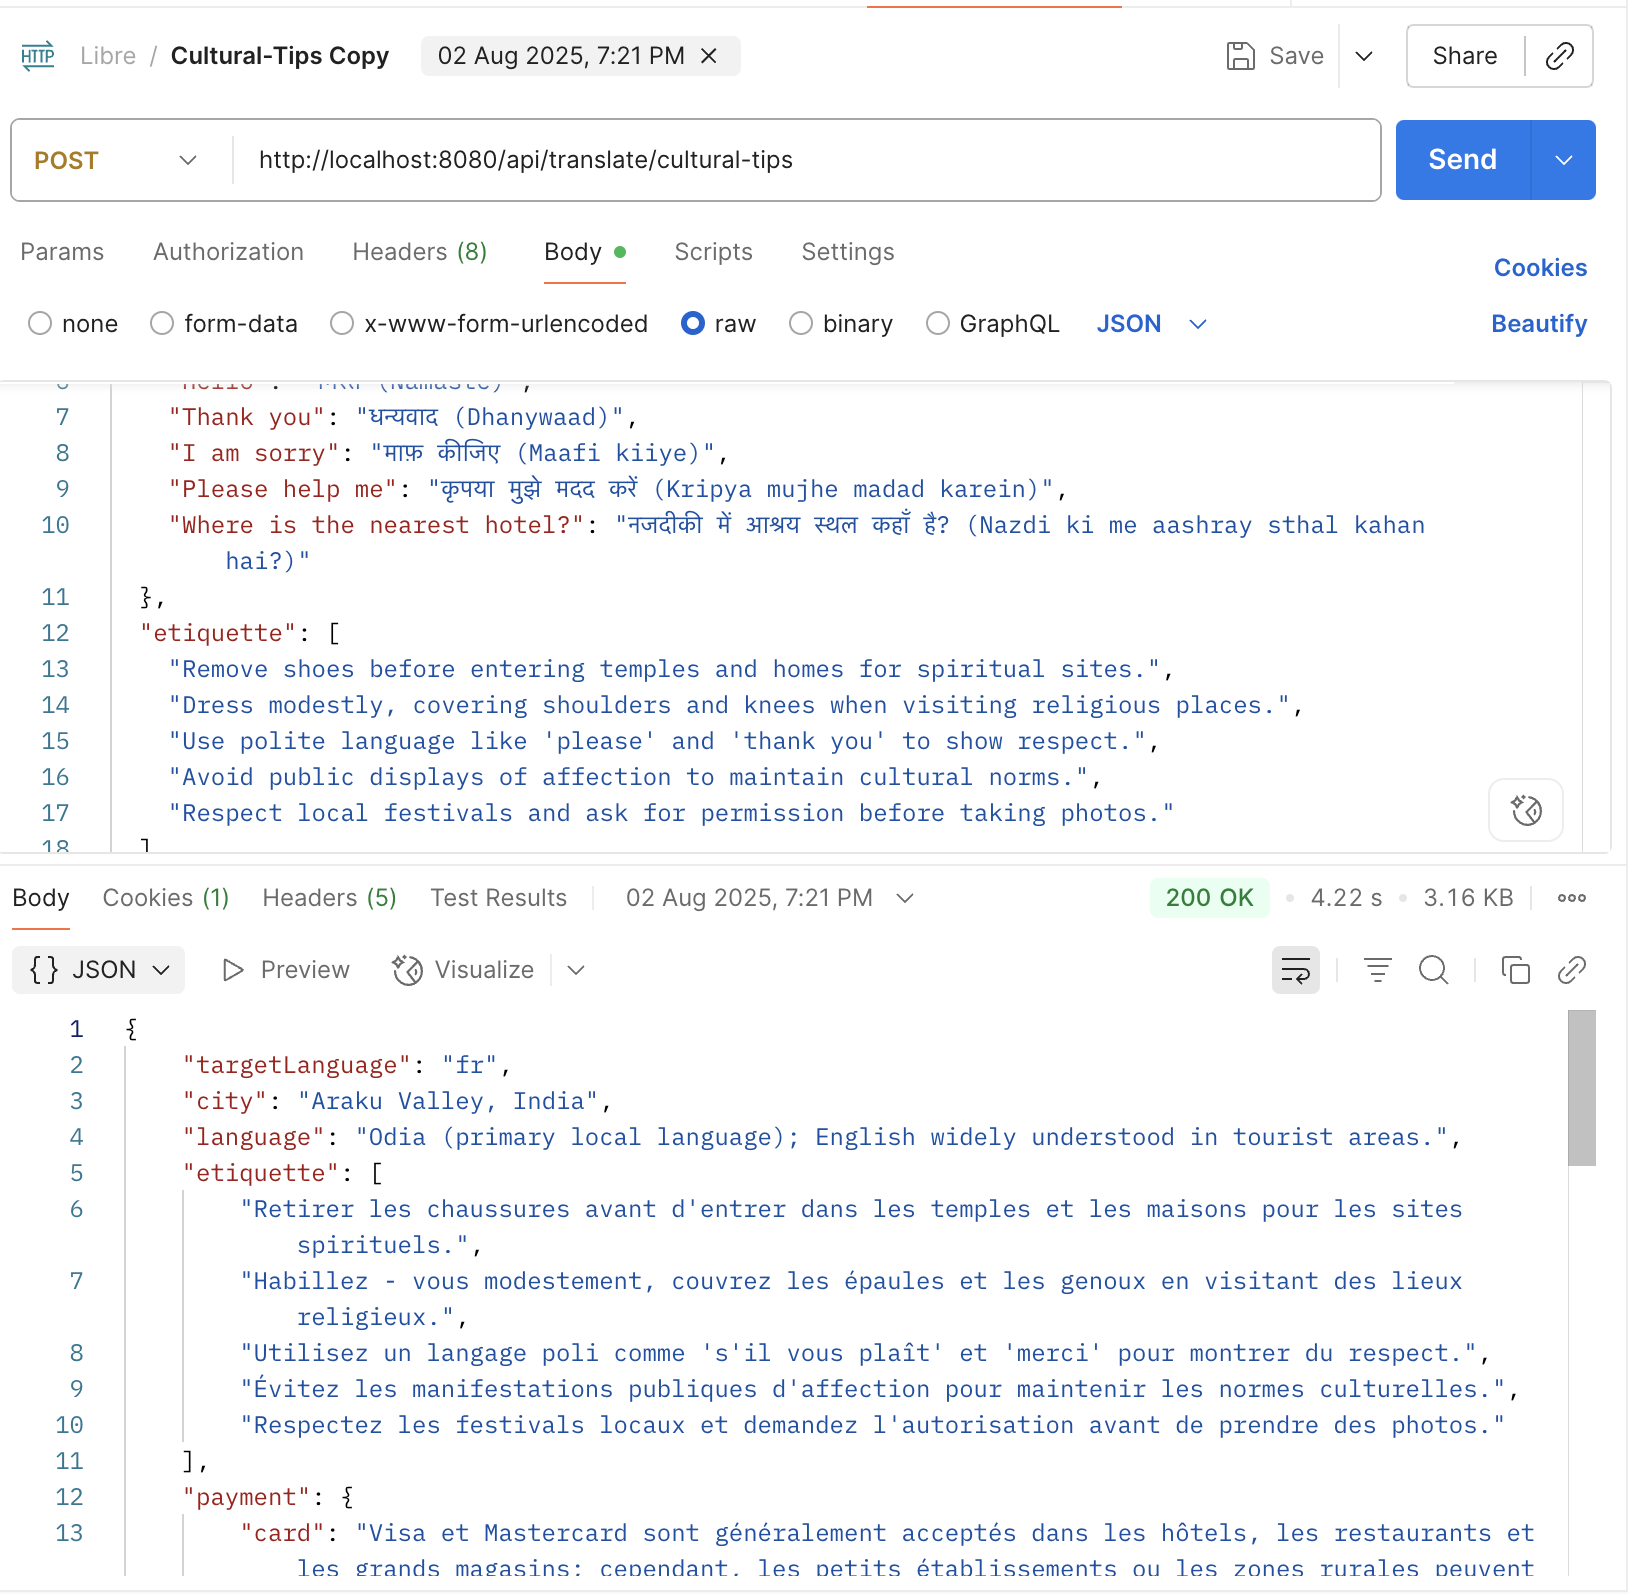
\includegraphics[width=1\linewidth]{images/Backend/Translation_Service_20_Red.png}
    \caption{The image shows an improvement from initial iteration of the backend implementation. The response times were down from 5.27s to 4.22s, a 20\% Reduction in Response Time.}
    \label{fig:20_reduction_response}
\end{figure}

\begin{figure}[H]
    \centering
    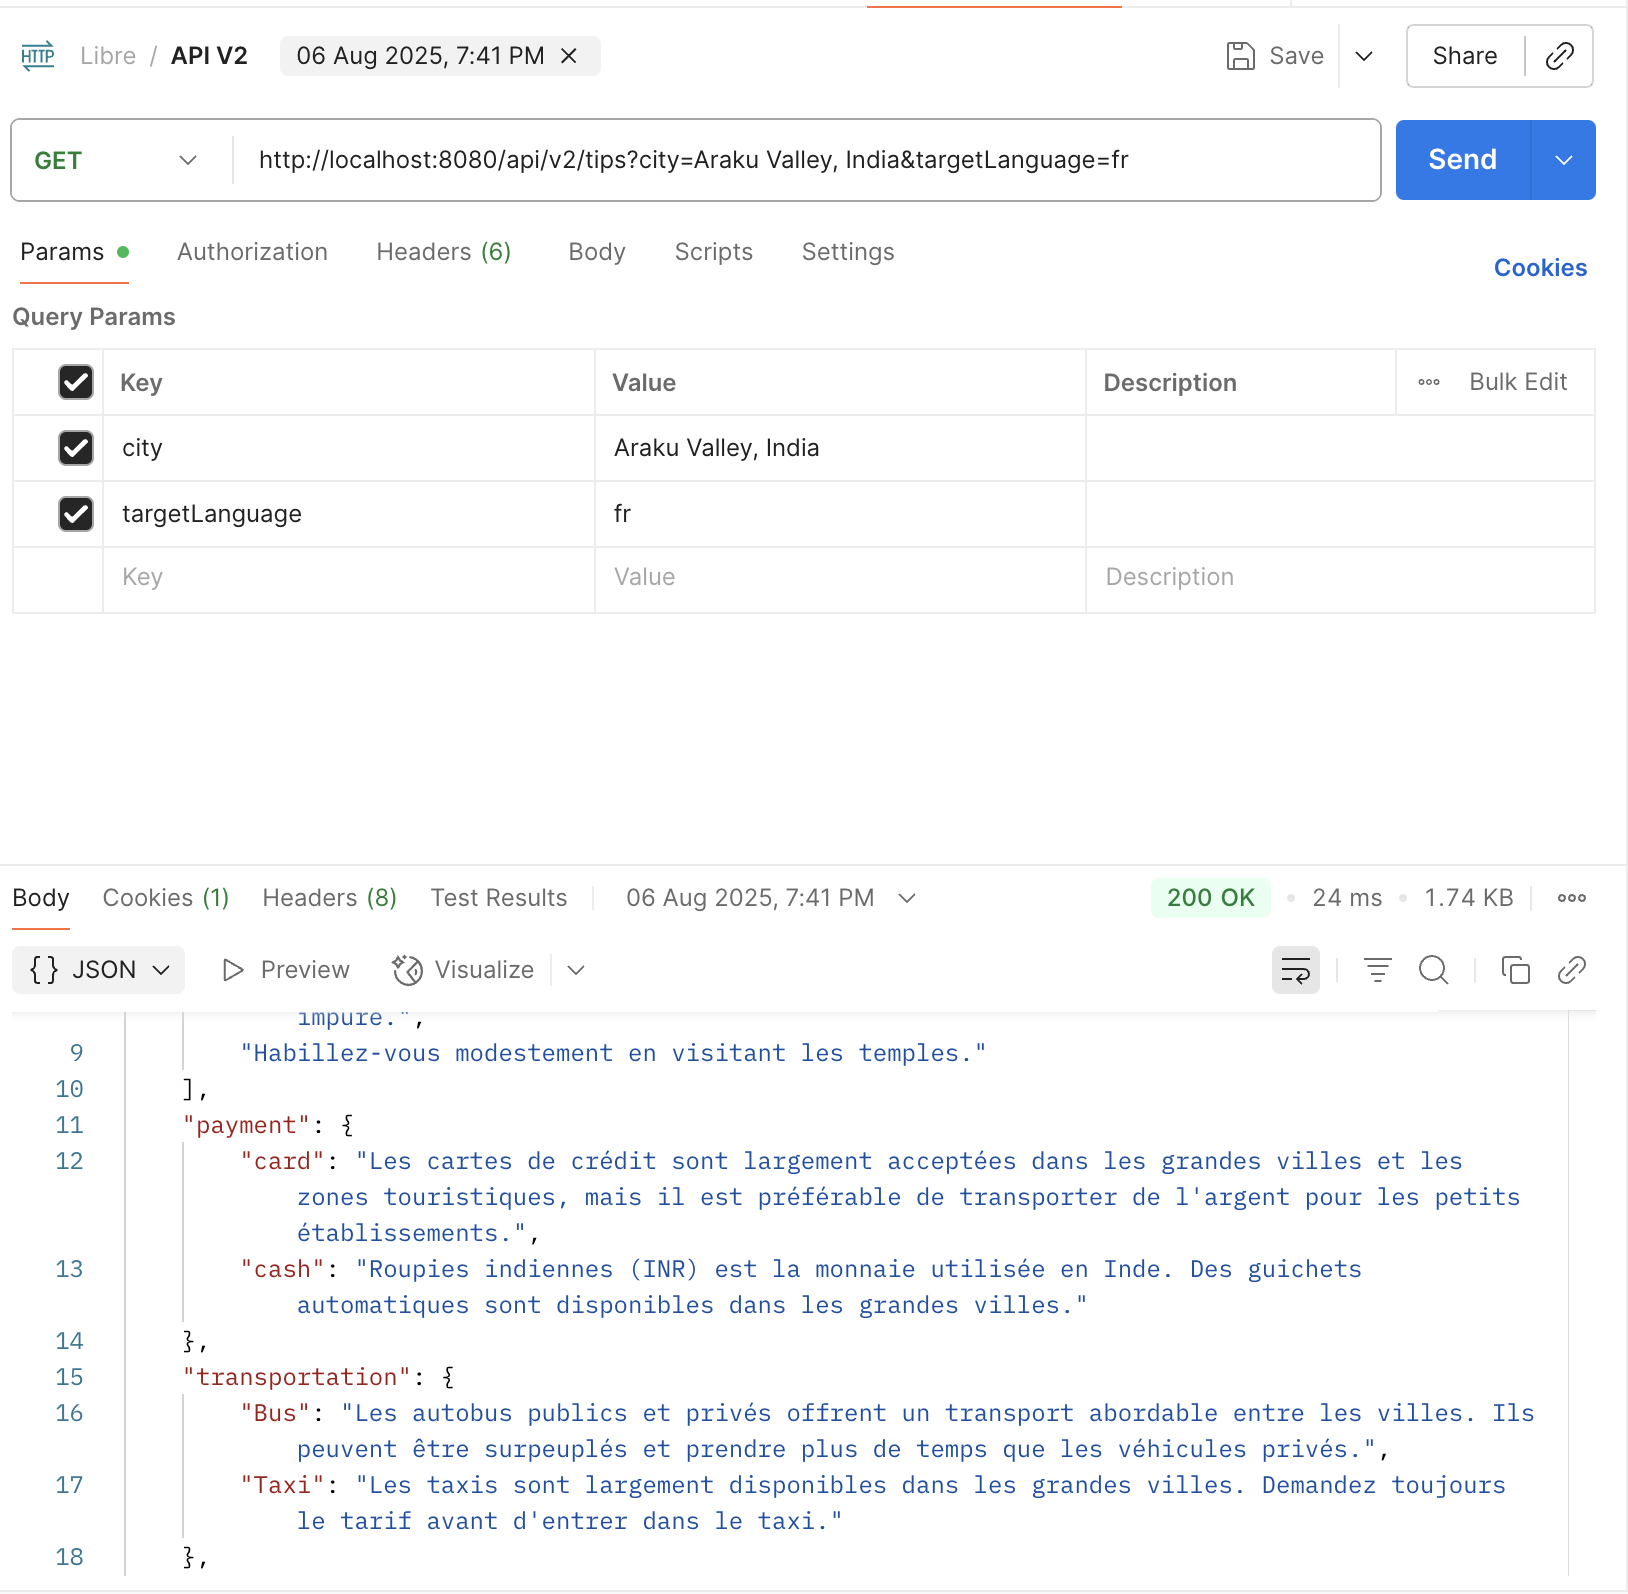
\includegraphics[width=1\linewidth]{images/Backend/Translation_Service_final_iteration.png}
    \caption{Final Response Time after implementing database as a cache layer to store cultural tips data. The image clearly shows a response time of 24ms fetched directly from database layer.}
    \label{fig:final_response_time}
\end{figure}

\begin{figure}[H]
    \centering
    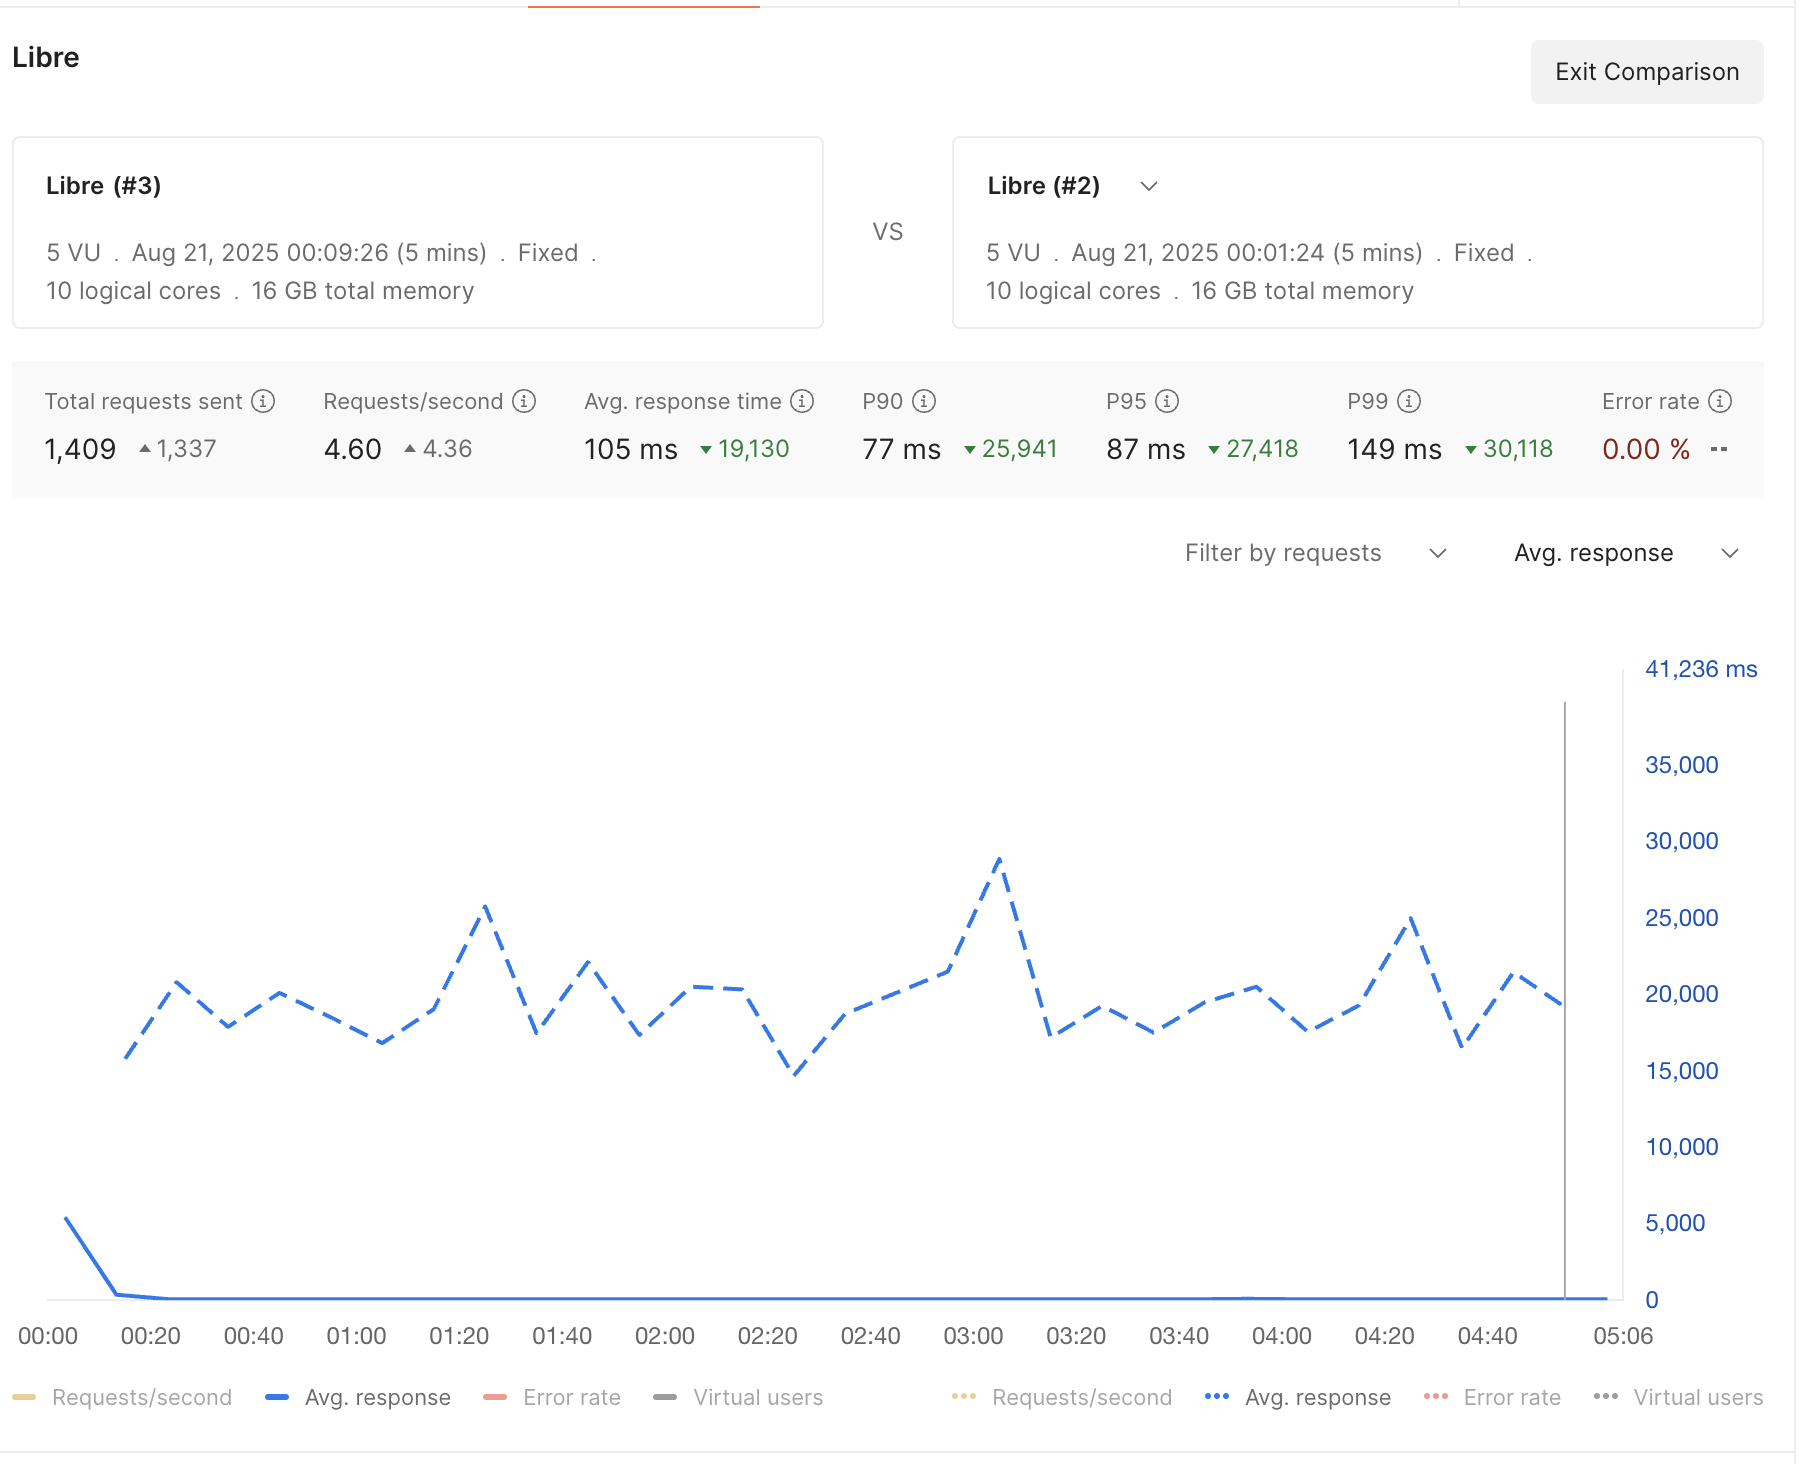
\includegraphics[width=1\linewidth]{images/Backend/Performance_Comparision.png}
    \caption{Performance comparison report of API version 1 (right side (Libre \#2) - avg. response shown in dotted blue line) and version 2 (left side (Libre \#3) - avg. response time shown in solid blue line). The graph clearly showing constant peaks in response time around 19,130ms, while version 2 showing an initial peak of 8000ms and then a steady performance around 105ms.}
    \label{fig:perf_comp}
\end{figure}